% Options for packages loaded elsewhere
\PassOptionsToPackage{unicode}{hyperref}
\PassOptionsToPackage{hyphens}{url}
%
\documentclass[
]{article}
\usepackage{amsmath,amssymb}
\usepackage{lmodern}
\usepackage{ifxetex,ifluatex}
\ifnum 0\ifxetex 1\fi\ifluatex 1\fi=0 % if pdftex
  \usepackage[T1]{fontenc}
  \usepackage[utf8]{inputenc}
  \usepackage{textcomp} % provide euro and other symbols
\else % if luatex or xetex
  \usepackage{unicode-math}
  \defaultfontfeatures{Scale=MatchLowercase}
  \defaultfontfeatures[\rmfamily]{Ligatures=TeX,Scale=1}
\fi
% Use upquote if available, for straight quotes in verbatim environments
\IfFileExists{upquote.sty}{\usepackage{upquote}}{}
\IfFileExists{microtype.sty}{% use microtype if available
  \usepackage[]{microtype}
  \UseMicrotypeSet[protrusion]{basicmath} % disable protrusion for tt fonts
}{}
\makeatletter
\@ifundefined{KOMAClassName}{% if non-KOMA class
  \IfFileExists{parskip.sty}{%
    \usepackage{parskip}
  }{% else
    \setlength{\parindent}{0pt}
    \setlength{\parskip}{6pt plus 2pt minus 1pt}}
}{% if KOMA class
  \KOMAoptions{parskip=half}}
\makeatother
\usepackage{xcolor}
\IfFileExists{xurl.sty}{\usepackage{xurl}}{} % add URL line breaks if available
\IfFileExists{bookmark.sty}{\usepackage{bookmark}}{\usepackage{hyperref}}
\hypersetup{
  pdftitle={Exploratory Cost-Effectiveness Analysis of Treatment Based on New Diagnostic Tests vs Standard of Care in Microsatellite Stable RAS Mutant Metastatic Colorectal Cancer Patients},
  pdfauthor={Jonathan Briody (1) \textbar{} Kathleen Bennett (1)},
  hidelinks,
  pdfcreator={LaTeX via pandoc}}
\urlstyle{same} % disable monospaced font for URLs
\usepackage[margin=1in]{geometry}
\usepackage{color}
\usepackage{fancyvrb}
\newcommand{\VerbBar}{|}
\newcommand{\VERB}{\Verb[commandchars=\\\{\}]}
\DefineVerbatimEnvironment{Highlighting}{Verbatim}{commandchars=\\\{\}}
% Add ',fontsize=\small' for more characters per line
\usepackage{framed}
\definecolor{shadecolor}{RGB}{248,248,248}
\newenvironment{Shaded}{\begin{snugshade}}{\end{snugshade}}
\newcommand{\AlertTok}[1]{\textcolor[rgb]{0.94,0.16,0.16}{#1}}
\newcommand{\AnnotationTok}[1]{\textcolor[rgb]{0.56,0.35,0.01}{\textbf{\textit{#1}}}}
\newcommand{\AttributeTok}[1]{\textcolor[rgb]{0.77,0.63,0.00}{#1}}
\newcommand{\BaseNTok}[1]{\textcolor[rgb]{0.00,0.00,0.81}{#1}}
\newcommand{\BuiltInTok}[1]{#1}
\newcommand{\CharTok}[1]{\textcolor[rgb]{0.31,0.60,0.02}{#1}}
\newcommand{\CommentTok}[1]{\textcolor[rgb]{0.56,0.35,0.01}{\textit{#1}}}
\newcommand{\CommentVarTok}[1]{\textcolor[rgb]{0.56,0.35,0.01}{\textbf{\textit{#1}}}}
\newcommand{\ConstantTok}[1]{\textcolor[rgb]{0.00,0.00,0.00}{#1}}
\newcommand{\ControlFlowTok}[1]{\textcolor[rgb]{0.13,0.29,0.53}{\textbf{#1}}}
\newcommand{\DataTypeTok}[1]{\textcolor[rgb]{0.13,0.29,0.53}{#1}}
\newcommand{\DecValTok}[1]{\textcolor[rgb]{0.00,0.00,0.81}{#1}}
\newcommand{\DocumentationTok}[1]{\textcolor[rgb]{0.56,0.35,0.01}{\textbf{\textit{#1}}}}
\newcommand{\ErrorTok}[1]{\textcolor[rgb]{0.64,0.00,0.00}{\textbf{#1}}}
\newcommand{\ExtensionTok}[1]{#1}
\newcommand{\FloatTok}[1]{\textcolor[rgb]{0.00,0.00,0.81}{#1}}
\newcommand{\FunctionTok}[1]{\textcolor[rgb]{0.00,0.00,0.00}{#1}}
\newcommand{\ImportTok}[1]{#1}
\newcommand{\InformationTok}[1]{\textcolor[rgb]{0.56,0.35,0.01}{\textbf{\textit{#1}}}}
\newcommand{\KeywordTok}[1]{\textcolor[rgb]{0.13,0.29,0.53}{\textbf{#1}}}
\newcommand{\NormalTok}[1]{#1}
\newcommand{\OperatorTok}[1]{\textcolor[rgb]{0.81,0.36,0.00}{\textbf{#1}}}
\newcommand{\OtherTok}[1]{\textcolor[rgb]{0.56,0.35,0.01}{#1}}
\newcommand{\PreprocessorTok}[1]{\textcolor[rgb]{0.56,0.35,0.01}{\textit{#1}}}
\newcommand{\RegionMarkerTok}[1]{#1}
\newcommand{\SpecialCharTok}[1]{\textcolor[rgb]{0.00,0.00,0.00}{#1}}
\newcommand{\SpecialStringTok}[1]{\textcolor[rgb]{0.31,0.60,0.02}{#1}}
\newcommand{\StringTok}[1]{\textcolor[rgb]{0.31,0.60,0.02}{#1}}
\newcommand{\VariableTok}[1]{\textcolor[rgb]{0.00,0.00,0.00}{#1}}
\newcommand{\VerbatimStringTok}[1]{\textcolor[rgb]{0.31,0.60,0.02}{#1}}
\newcommand{\WarningTok}[1]{\textcolor[rgb]{0.56,0.35,0.01}{\textbf{\textit{#1}}}}
\usepackage{graphicx}
\makeatletter
\def\maxwidth{\ifdim\Gin@nat@width>\linewidth\linewidth\else\Gin@nat@width\fi}
\def\maxheight{\ifdim\Gin@nat@height>\textheight\textheight\else\Gin@nat@height\fi}
\makeatother
% Scale images if necessary, so that they will not overflow the page
% margins by default, and it is still possible to overwrite the defaults
% using explicit options in \includegraphics[width, height, ...]{}
\setkeys{Gin}{width=\maxwidth,height=\maxheight,keepaspectratio}
% Set default figure placement to htbp
\makeatletter
\def\fps@figure{htbp}
\makeatother
\setlength{\emergencystretch}{3em} % prevent overfull lines
\providecommand{\tightlist}{%
  \setlength{\itemsep}{0pt}\setlength{\parskip}{0pt}}
\setcounter{secnumdepth}{-\maxdimen} % remove section numbering
\ifluatex
  \usepackage{selnolig}  % disable illegal ligatures
\fi
\newlength{\cslhangindent}
\setlength{\cslhangindent}{1.5em}
\newlength{\csllabelwidth}
\setlength{\csllabelwidth}{3em}
\newenvironment{CSLReferences}[2] % #1 hanging-ident, #2 entry spacing
 {% don't indent paragraphs
  \setlength{\parindent}{0pt}
  % turn on hanging indent if param 1 is 1
  \ifodd #1 \everypar{\setlength{\hangindent}{\cslhangindent}}\ignorespaces\fi
  % set entry spacing
  \ifnum #2 > 0
  \setlength{\parskip}{#2\baselineskip}
  \fi
 }%
 {}
\usepackage{calc}
\newcommand{\CSLBlock}[1]{#1\hfill\break}
\newcommand{\CSLLeftMargin}[1]{\parbox[t]{\csllabelwidth}{#1}}
\newcommand{\CSLRightInline}[1]{\parbox[t]{\linewidth - \csllabelwidth}{#1}\break}
\newcommand{\CSLIndent}[1]{\hspace{\cslhangindent}#1}

\title{Exploratory Cost-Effectiveness Analysis of Treatment Based on New
Diagnostic Tests vs Standard of Care in Microsatellite Stable RAS Mutant
Metastatic Colorectal Cancer Patients}
\author{Jonathan Briody (1) \textbar{} Kathleen Bennett (1)}
\date{}

\begin{document}
\maketitle

\begin{enumerate}
\def\labelenumi{(\arabic{enumi})}
\tightlist
\item
  Data Science Centre, RCSI University of Medicine and Health Sciences,
  Dublin, Ireland
\end{enumerate}

\hypertarget{abstract}{%
\section{\texorpdfstring{\textbf{Abstract:}}{Abstract:}}\label{abstract}}

\textbf{Background:} Colorectal cancer is the third most common cancer
in Europe. Microsatellite stable RAS mutant metastatic colorectal cancer
(MSS RAS mt mCRC). \textbf{Objectives:} The objective of this study was
to compare the cost-effectiveness of a personalised medicine approach
(evaluation of predictive biomarkers for targeted therapy) with standard
of care treatment FOLFOX (5-FU, leucovorin, and oxaliplatin) in patients
with MSS RAS mt mCRC in Germany, Ireland and Spain.

\textbf{Materials and Methods:} We developed a three-state Markov model
with monthly cycles to estimate the incremental cost-effectiveness ratio
(ICER) of biomarkers for targeted therapies versus FOLFOX for patients
with mCRC from a healthcare payer perspective in the countries under
study (Germany, Ireland and Spain). Progression risks, cause-specific
mortality and probabilities of adverse events were taken from the
literature. Costs for treatment administration and management of adverse
events were derived from published data and survey of consortium
hospitals in the countries participating. Utilities applied to calculate
the quality-adjusted life years (QALYs) were obtained from a review of
the literature {[}I may want to return to this to update this with the
country specific utility plan myself and Kathleen made{]}. To test the
robustness of the results one-way sensitivity analysis and probabilistic
sensitivity analysis was applied.

\textbf{Results:} Predictive biomarkers with targeted therapy provided X
QALYS at a cost of €X,000 compared with standard of care (FOLFOX without
testing). Compared to standard of care, the ICER of predictive
biomarkers with targeted therapy provided was EUR X,000/QALY from a
European health care perspective, which was above the threshold used to
define cost-effectiveness in the countries studied, which provided X
QALYS at a cost of €X,000. The incremental cost-effectiveness ratio
(ICER) was €X,000 per QALY. The ICER was below the cost-effectiveness
threshold (\textless€X,000 per QALY) in all univariate and multivariate
sensitivity analyses. One-way sensitivity analysis demonstrated that the
initial results were generally robust. Cost-effectiveness acceptability
curves from the probabilistic sensitivity analysis show that the
probability that predictive biomarkers with targeted therapy was
cost-effective was 100\% when the threshold was \textless€X,000 per
QALY.

\textbf{Conclusion:} When compared to standard of care, predictive
biomarkers with targeted therapy is cost effective for patients with MSS
RAS mt mCRC in Germany, Ireland and Spain at a €X,000 per QALY
threshold. However, because of the exploratory nature of this analysis,
the cost effectiveness profile of these biomarkers should be evaluated
in further comparative studies.

\textbf{Keywords:} Colorectal neoplasms, cost effectiveness analysis,
Quality-adjusted life years, Markov model, mCRC, precision medicine,
biomarkers, assays,

JEL CLASSIFICATION CODES

I19, I1, I, I11, I1, I,

\underline{\emph{Possible Journal Homes:}}

Value in Health: BEST POSSIBLE HOME, HIGHEST RATED JOURNAL, FOCUSED ON
CEA, ETC.,

Journal of Medical Economics
\url{https://www.tandfonline.com/doi/pdf/10.1080/13696998.2021.1888743}

Clinical Colorectal Cancer
\url{https://www-sciencedirect-com.proxy.library.rcsi.ie/science/article/pii/S1533002814000978}

\textbf{Correspondence:}

Jonathan Briody, PhD, RCSI University of Medicine and Health Sciences,
Beaux Lane House, Lower Mercer St, Dublin 2, Ireland. Email:
\href{mailto:jonathanbriody@rcsi.ie}{\nolinkurl{jonathanbriody@rcsi.ie}}

\textbf{Funding Information:}

This project has received funding from the European Union's Horizon 2020
research and innovation programme under grant agreement No 754923. The
material presented and views expressed here are the responsibility of
the author(s) only. The EU Commission takes no responsibility for any
use made of the information set out.

\newpage

\hypertarget{introduction}{%
\section{Introduction}\label{introduction}}

With almost 2 million new cases diagnosed annually, colorectal cancer is
the third most commonly diagnosed cancer in men, the second most
commonly diagnosed in women (Vabi, Gibbs, and Parker 2021), and the
second leading cause of cancer deaths worldwide (Nwaokorie and Fey
2021). Following advances in primary and adjuvant treatments, survival
time continues to improve in colorectal cancer, with a 5-year survival
rate of 64\%, however, this is not reflected in metastatic colorectal
cancer (mCRC), which has a dramatically lower 5-year survival rate of
just 12\% (Siegel, Miller, and Jemal 2019).

As one of the most commonly mutated oncogenes in cancer, RAS mutations
appear in around half of mCRC patients, and in microsatellite stable
(MSS) mCRC are associated with more aggressive tumor biology and poorer
prognosis (Patelli et al. 2021). Current front-line treatment for mCRC
does not differ significantly from colorectal cancer regardless of
mutational status, comprising of 5-fluoruracil (5-FU)-based standard of
care chemotherapy (e.g.~FOLFOX, FOLFIRI, FOLFOXFIRI) in combination with
bevacizumab. However, there is emerging evidence that targeted therapy
may prolong overall survival for mCRC patients, as previously seen in
non-metastatic colorectal cancer (Xie, Chen, and Fang 2020).

Cancerous cells may be addressed by targeted therapy which directly
inhibits cell proliferation, differentiation, and migration. Similarly,
the micro-environment of the tumor, including it's local blood vessels
and immune cells, may be modified in order to disrupt growth and to
improve immune surveillance and response (Tiwari et al. 2018). Beginning
with Cetuximab in 2004, numerous targeted therapies for colorectal
cancer have successfully come to market in the last two decades
(Bevacizumab, Panitumumab, Ziv-aflibercept, Regorafenib, Ramucirumab,
Pembrolizumab, Bivolumabm Ipilimumab, etc.,). The number of pathways
offering possible opportunities for targeted therapy is similarly
extensive, including epidermal growth factor receptor (EGFR), vascular
endothelial growth factor/vascular endothelial growth factor receptor
(VEGF/VEGFR), and hepatocyte growth factor/mesenchymal--epithelial
transition factor (HGF/c-MET), among others (Xie, Chen, and Fang 2020).

\emph{DRUG X} is a \emph{DETAILS ABOUT DRUG X HERE} that \emph{HOW DRUG
X WORKS HERE} {[}citation to support this{]}. This experimentally
identified targeted agent is in preclinical status or in phase I trials,
but has been proven to be efficient in clinical studies {[}amend if this
isnt the case{]}, and \ldots{} {[}citations to support this{]}. The
results of X demonstrate a median overall survival (OS) benefit of X
months (Y months vs.~Z months) and a median progression-free survival
(PFS) benefit of X months for DRUG X when compared with placebo (X
months vs.~X months).

\begin{quote}
Fruquintinib is a VEGFR inhibitor that blocks new blood vessel growth
associated with tumor proliferation5 . In 2018, it was approved to treat
Chinese patients with mCRC who had experienced failure of second-line
treatment. The results of the FRESCO trial demonstrated a median overall
survival (OS) benefit of 2.7 months (9.3 months vs.~6.6 months) and a
median progression-free survival (PFS) benefit of 1.9 months for
fruquintinib when compared with placebo (3.7 months vs.~1.8 months)6.

- Guan, X., Li, H., Xiong, X., Peng, C., Wang, N., Ma, X., \& Ma, A.
(2021). Cost-effectiveness analysis of fruquintinib versus regorafenib
as the third-line therapy for metastatic colorectal cancer in China.
\emph{Journal of Medical Economics}, \emph{24}(1), 339-344.
\end{quote}

Because targeted therapy is most associated with prolonged survival,
rather than cure, the cost--effectiveness of such therapy must be
understood when compared to current standard of care chemotherapy, which
is assumed to be significantly less costly than producing targeted
agents and testing necessary genetic markers, particularly under the
provision of multiple targeted agents (Dekker et al. 2019).

Limited data exist regarding these novel therapies, with no research
comparing the cost-effectiveness of these targetted therapies with
standard of care, thus, we developed a general decision-analytic
framework applied to mCRC to model the cost-effectiveness of biomarkers
for targeted therapies in mCRC. We constructed a Markov model using a
hypothetical cohort of patients with mCRC to conduct an exploratory
cost-effectiveness analysis of targeted treatment based on new
diagnostic tests vs standard of care in MSS RAS mt mCRC patients.

\hypertarget{materials-and-methods}{%
\section{Materials and Methods}\label{materials-and-methods}}

\hypertarget{model-structure}{%
\paragraph{Model Structure}\label{model-structure}}

We constructed Markov models to calculate the lifetime costs and
outcomes of each treatment strategy. As per Figure 1, in this model we
established the following health states: (1) first line treatment prior
to progression; (2) second line treatment following progression; (3)
death. We applied published estimates of costs associated with each
health state in the countries studied {[}CITE{]}. All cost estimates
were in 2022 Euros {[}maybe discuss how you converted to this? HIQA has
something on this I think{]}. To apply country-specific state utility
values we\ldots DETAIL HERE THE APPROACH WE TOOK AS DISCUSSED WITH
KATHLEEN {[}CITE{]}. The model was programmed in R 4.1.2 using RStudio
2021.09.2+382 and was informed by the state-transition model framework
developed by the Decision Analysis in R for Technologies in Health
(DARTH) workgroup (Alarid-Escudero et al. 2021) (Jalal et al. 2017)
(Krijkamp et al. 2018) (Krijkamp et al. 2020). The Markov model
simulated the health state transitions following a diagnosis of
metastatic cancer. A cycle length of 1 month was chosen, per the time
between administration of chemotherapy doses. A 5-year time horizon was
also chosen {[}CITE{]}. For standard of care, we considered 2 lines of
treatment, first line (FOLFOX) and second line (FOLFIRI). For the
comparator we also considered 2 lines of treatment (NEW THERAPY), then
(FOLFIRI). In both instances we made use of treatment-specific utility
values. At the end of each cycle, patients remained in their current
health state, or transitioned to a more progressive state. To reflect
that transitions between states may occur at any point within each
cycle, we applied a half-cycle correction to calculating life-years
(LYs) \{I AM DEFINITELY NOT GOING TO DO THIS, I JUST PUT IT IN HERE AS
SOMETHING TO THINK ABOUT, CYCLES ARE ONLY A MONTH SO A CORRECTION OF 2
WEEKS IS PRETTY STUPID\}.

\begin{quote}
{[}A three-state Markov model (Figure 1) with monthly cycle could also
have been used to represent the progression of mCRC, including PFS,
progressive disease (PD), and death. All patients entered the model
either receiving FOLFOX therapy or NOVEL therapy. After treatment
discontinuation due to progession, best supportive care (BSC) was
modeled. **--\textgreater{} So, here even doing that they still got a
treatment that needs to be modelled in PFS{]}.**

Guan, X., Li, H., Xiong, X., Peng, C., Wang, N., Ma, X., \& Ma, A.
(2021). Cost-effectiveness analysis of fruquintinib versus regorafenib
as the third-line therapy for metastatic colorectal cancer in China.
\emph{Journal of Medical Economics}, \emph{24}(1), 339-344.
\end{quote}

The intention-to-treat (ITT) population we modeled in this study is MSS
RAS mt mCRC patients in Germany, Ireland and Spain, from a healthcare
payer perspective in these countries. Subsequently the analysis only
included direct medical costs. Effectiveness is reflected in life-years
(LYs) and quality adjusted life years (QALYS). Per the countries
studied, a discount rate of 4\% per annum was applied to cost input and
health output parameters {[}citation here{]}. The primary outcome of the
model was the total direct costs, LYs, QALYS, and the incremental
cost-effectiveness ratio (ICER).

\hypertarget{patients-and-treatment-regimens}{%
\paragraph{Patients and Treatment
Regimens}\label{patients-and-treatment-regimens}}

In the absence of a randomised controlled trial making direct
comparisons between standard of care and the proposed novel therapy, it
was necessary to perform an indirect comparison using the data from two
published studies {[}CITE{]}. We made use of published results from one
study to estimate the clinical course for patients treated under
standard of care and another to estimate outcomes for patients under
novel therapy (Goldstein et al. 2014). The standard of care arm was
based on a study be ..et al., \{FILL IN THE BLANKS HERE ON THE STUDY YOU
BASED THIS ON\} who compared\ldots{[}cite{]}. The novel therapy arm was
based on a X, Y, Z, study by \ldots.et al., While these 2 studies did
not have identical target populations\ldots{}

\begin{quote}
The PK arm was based on a phase II nonrandomized study by Capitain et
al., who compared PK FOLFOX with BSA FOLFOX.9 The BSA arm was based on a
phase III randomized study by Tournigand et al.14 Although the 2 studies
did not have identical target populations, the survival outcomes of the
baseline BSA arm of the 2 studies are comparable (Table 1).9,14,15
Moreover, the median PFS and OS were also similar to the FOLFOX arm in a
similar study.15

Goldstein, D. A., Chen, Q., Ayer, T., Howard, D. H., Lipscomb, J.,
Harvey, R. D., \ldots{} \& Flowers, C. R. (2014). Cost effectiveness
analysis of pharmacokinetically-guided 5-fluorouracil in FOLFOX
chemotherapy for metastatic colorectal cancer. \emph{Clinical colorectal
cancer}, \emph{13}(4), 219-225.

Given that there was no single RCT with all treatment arms, it was
necessary to perform an indirect comparison using the data from the
FRESCO trial and the CONCUR trial6, 11. The baseline treatment for the
indirect comparison was BSC taken from the FRESCO trial. The clinical
effectiveness in patients in the BSC arm was also available from the
CONCUR trial. This, however, was not considered appropriate for the
baseline treatment because the survival curves reported by the CONCUR
trial were distorted in the paper and were not suitable for recreating
individual patient data. However, the hazard ratios (HRs) calculated by
original data would not be affected by the distorted figures. The
implicit assumption underlying the indirect comparison was that the
baseline patient characteristics in the two studies were reasonably
similar, which was shown to be true (Appendix Table 1).

The FRESCO trial was used to model the probabilities of remaining in the
PFS state or experiencing disease progression in the fruquintinib arm.
This research recreating individual patients data (IPD) from
Kaplan--Meier (KM) survival curves in FRESCO by the method published by
Guyot et al.12. To predict the events of death and progression beyond
the observation period, several parametric models were fit in different
distributions, including exponential, Weibull, Gompertz, generalized
gamma log-normal and log-logistic. After comparing the goodness-of-fit
of different parametric models by the Akaike information criterion (AIC)
and the Bayesian information criterion (BIC) (Appendix Table 2),
assessing the conformities of parametric models to the original KM
survival curves in the FRESCO trial and considering about proportional
hazard model used for the indirect comparison, the Weibull distribution
model was chosen for the base case analysis (Appendix Figure 1 and
Appendix Figure 2).

We used the PFS curves to estimate the transition probability from PFS
state to PFS state and the transition probability from PFS state to
another states (PD and death) and used the OS curve to estimate the
overall mortality. The model assumed the transition probability from PFS
state to death was estimated by the background mortality obtained from
Chinese government data, which based on actuarial estimates of mortality
among the general population in China. According to the background
mortality and the transition probability from PFS state to another
states (PD and death), we calculated the transition probability from PFS
state and PD. Moreover, the transition probability from PD state to PD
state could calculated by overall mortality and background mortality.

We also calculated the transition probabilities in the BSC arm by a
Weibull-distribution hazard function using the survival data from the
FRESCO trial. The model assumed that the survival curves of BSC both in
FRESCO and CONCUR would be identical if the patients in BSC arm was
identical, and the HR of regorafenib versus BSC would not change even if
the patients receiving BSC in CONCUR became exactly same as the patients
receiving BSC in FRESCO. Hence,we adjusted the transition probabilities
of the regorafenib arm using the transition probabilities of the BSC arm
modeled from the FRESCO trial and the HR of regorafenib versus BSC taken
from the CONCUR trial.

Guan, X., Li, H., Xiong, X., Peng, C., Wang, N., Ma, X., \& Ma, A.
(2021). Cost-effectiveness analysis of fruquintinib versus regorafenib
as the third-line therapy for metastatic colorectal cancer in China.
\emph{Journal of Medical Economics}, \emph{24}(1), 339-344.
\end{quote}

\begin{quote}
There is a discussion on indirect comparisons and how best to do these
in this short piece: Martin-Broto, J. (2015). Indirect comparisons in
cost-effectiveness analysis: are we being naïve?. Clinical and
Translational Oncology, 17(1), 85-86.
\url{https://sci-hub.se/10.1007/s12094-014-1256-9}

This also talks about indirect comparisons Hollmann, S., Alloul, K.,
Attard, C., \& Kavan, P. (2014). An Indirect Treatment Comparison and
Cost-Effectiveness Analysis Comparing Folfirinox with Nab-Paclitaxel
Plus Gemcitabine for First-Line Treatment for Patients with Metastatic
Pancreatic Cancer. Annals of Oncology, 25, ii11.
\url{https://sci-hub.se/10.1093/annonc/mdu164.18}

This applies an indirect comparison in more detail: Tamoschus, D.,
Draexler, K., Chang, J., Ngai, C., Madin-Warburton, M., \& Pitcher, A.
(2017). Cost-effectiveness analysis of regorafenib for gastrointestinal
stromal tumour (GIST) in Germany. Clinical Drug Investigation, 37(6),
525-533. \url{https://sci-hub.se/10.1007/s40261-017-0514-3}

I'm not even sure if I would classify what we are doing as an indirect
comparison, as we don't have data for the novel therapy at all (that I
know of), but I'll read the above articles and then make a call on that.

The following also shows how to do the above: Purmonen, T., Martikainen,
J. A., Soini, E. J., Kataja, V., Vuorinen, R. L., \&
Kellokumpu-Lehtinen, P. L. (2008). Economic evaluation of sunitinib
malate in second-line treatment of metastatic renal cell carcinoma in
Finland. Clinical therapeutics, 30(2), 382-392. -
\url{https://sci-hub.se/10.1016/j.clinthera.2008.02.013}

\textbf{\emph{Or we could try:}}

The transition probabilities were derived from the median time to
radiologic progression and median OS obtained from previously published
studies18,20 following recommended methods21. - Per: Hamdy Elsisi, G.,
Nada, Y., Rashad, N., \& Carapinha, J. (2019). Cost-effectiveness of
sorafenib versus best supportive care in advanced hepatocellular
carcinoma in Egypt. Journal of Medical Economics, 22(2), 163-168.
\url{https://www-tandfonline-com.proxy.library.rcsi.ie/doi/pdf/10.1080/13696998.2018.1552432}
\end{quote}

\hypertarget{transition-probabilities}{%
\paragraph{Transition Probabilities}\label{transition-probabilities}}

\begin{quote}
Progression Risk and Mortality Progression risks and cause-specific
mortalities for each arm were derived from the PFS and OS curves of the
corresponding study. Engauge Digitizer16 was used to extract the data
points from each PFS and OS plot, and then used to fit parametric
survival models. Statistical analyses demonstrated that Weibull and
log-logistic models provided a good fit for all curves according to the
Akaike information criterion, Schwarz Bayesian criterion,17 and visual
inspection (Supplemental Table 1 in the online version). Weibull models
permit the hazard rate to increase over time and are thus more suitable
for modeling events occurring early during follow-up periods. We
therefore selected the Weibull model for all survival curves in this
analysis. Next, we estimated the risk for each cycle based on the fitted
survival models. In particular, because OS is defined as the period
between the start of treatment and death, we computed the cause-specific
mortality rates, p1(t), at cycle t based on the fitted Weibull OS model,
OS(t), using the formula:

p1ðtÞ ¼ Pðt T t þ 1Þ PðT tÞ ¼ ðOSðtÞ  OSðt  1ÞÞ OSðtÞ : (1)

PFS is the period between the start and progression of disease or death.
We computed the combined risks p2(t) based on the Weibull PFS model
using Formula 1 and computed p2(t)  p1(t) as the estimate of the
progression risks. Estimates of mortality and progression risk beyond
the follow-up time in the clinical trials were extrapolated based on the
fitted survival models. The overall mortality was defined according to
the maximum value of cause-specific mortality and the background
mortality. We use the US life tables to estimate the background
mortality for each age group separately.18 In each run of the model
simulation, the initial age was sampled from the distribution of age at
diagnosis for mCRC in the Surveillance, Epidemiology, and End Results
database since the year 2000.

Goldstein, D. A., Chen, Q., Ayer, T., Howard, D. H., Lipscomb, J.,
Harvey, R. D., \ldots{} \& Flowers, C. R. (2014). Cost effectiveness
analysis of pharmacokinetically-guided 5-fluorouracil in FOLFOX
chemotherapy for metastatic colorectal cancer. \emph{Clinical colorectal
cancer}, \emph{13}(4), 219-225.

I discussed parametric survival analysis with Andy here:
C:\textbackslash Users\textbackslash Jonathan\textbackslash OneDrive -
Royal College of Surgeons in
Ireland\textbackslash COLOSSUS\textbackslash Training
Resources\textbackslash Decision Modelling - Advanced
Course\textbackslash A1\_Advanced Markov Modelling\textbackslash A1.3
Practical exercise R
\end{quote}

\textbf{{[}So, I think my takeway is that I need to do digitising and
maybe parametric survival analysis on some existing published data - per
C:\textbackslash Users\textbackslash Jonathan\textbackslash OneDrive -
Royal College of Surgeons in
Ireland\textbackslash COLOSSUS\textbackslash Parametric Survival
Analysis and the rest of my York training material THEN I'll need to
include Age specific all cause mortality per:
C:\textbackslash Users\textbackslash Jonathan\textbackslash OneDrive -
Royal College of Surgeons in
Ireland\textbackslash COLOSSUS\textbackslash Training
Resources\textbackslash Cost-Effectiveness and Decision Modeling using R
Workshop \_ DARTH because I don't have my own clinical data, these are
both good sources to consider seeing as they also didnt have their own
data, I'll also have to think about the age of the cohort if I include
competing mortality, as below:{]}.}

\begin{quote}
``Starting age of the cohort was 60 years, which is the median age of
incident breast cancer cases as reported by The Netherlands Cancer
Registration {[}28{]}.'' per: Kip, M., Monteban, H., \& Steuten, L.
(2015). Long-term cost--effectiveness of Oncotype DX® versus current
clinical practice from a Dutch cost perspective. Journal of comparative
effectiveness research, 4(5), 433-445.
C:/Users/Jonathan/Dropbox/PC/Downloads/kip2015\%20(1).pdf

``Nonbreast cancer death was captured as a competing risk in the model.
These data were derived from The Netherlands Cancer Registration and
based on Dutch female life tables for 2007--2009 {[}28,33{]}. Kip, M.,
Monteban, H., \& Steuten, L. (2015). Long-term cost--effectiveness of
Oncotype DX® versus current clinical practice from a Dutch cost
perspective. Journal of comparative effectiveness research, 4(5),
433-445.''
\url{file:///C:/Users/Jonathan/Dropbox/PC/Downloads/kip2015\%20(1).pdf}

Patients had a starting age of 56 years Salem, A., Men, P., Ramos, M.,
Zhang, Y. J., Ustyugova, A., \& Lamotte, M. (2021). Cost--effectiveness
analysis of empagliflozin compared with glimepiride in patients with
Type 2 diabetes in China. \emph{Journal of Comparative Effectiveness
Research}, \emph{10}(6), 469-480.
\end{quote}

\hypertarget{utility-estimates}{%
\paragraph{Utility Estimates}\label{utility-estimates}}

To present health outcomes in terms of QALYS, we adjusted survival time
by quality of life using a Health Related Quality of Life (HR-QOL) score
on a 0-1 utility scale. The quality of life utilities of a cycle spent
in each of the model health states has been estimated to be 0.85 for the
first line health state, and 0.65 for the second line health state in
the published literature on quality of life utility of patients with
mCRC without complications (Ramsey et al. 2000) {[}We want to be clear,
per Craig, D., McDaid, C., Fonseca, T., Stock, C., Duffy, S., \&
Woolacott, N. (2009). Are adverse effects incorporated in economic
models? An initial review of current practice. \emph{Health Technology
Assessment (Winchester, England)}, \emph{13}(62), 1-71., that our
utilities come from patients without adverse events, otherwise the
disutilty of these adverse events have already been counted, so we want
utility before any adverse events occur, and then we can decrease this
with disutility for these adverse events per the studies AND MAYBE
EXPLAIN MY PLAN WITH KATHLEEN HERE TO GET COUNTRY SPECIFIC UTILITY
VALUES{]}. We assumed in the model that utility was only related to
health state, and not to therapy.

\begin{quote}
We established the probability of Grade 3 and 4 adverse events (AEs)
from the trials used for the models.15,20 Goldstein, D. A., Chen, Q.,
Ayer, T., Howard, D. H., Lipscomb, J., Harvey, R. D., \ldots{} \&
Flowers, C. R. (2014). Cost effectiveness analysis of
pharmacokinetically-guided 5-fluorouracil in FOLFOX chemotherapy for
metastatic colorectal cancer. \emph{Clinical colorectal cancer},
\emph{13}(4), 219-225.

To do this, they basically went to the studies by:

Capitain et al, 2012

Hochster et al, 2008

Bennouna et al, 2013

And went to the tables on ``Incidence of Grade X and Grade Y Adverse
Events,'' and took the percentages reported in these studies to use in
their own table under ``Adverse Event Incidence''

Then, according to:
\href{https://en.wikipedia.org/wiki/Incidence_(epidemiology)}{{[}https://en.wikipedia.org/wiki/Incidence\_(epidemiology{]}(https://en.wikipedia.org/wiki/Incidence\_(epidemiology))}
because we have explicitly something called an ``incidence'' we are
allowed use this as a probability in our analysis, so, having filled in
the ``Adverse Event Incidence'' section in our Table on model parameters
like they do, we can then use these ``incidence'' values as
probabilities.

Remember that Leukopenia = Febrile Neutropenia.
\end{quote}

The probability of Grade 3/4 adverse events (AEs) was informed by the
literature {[}CITE{]}.

AEs can reduce patients' utility so we applied disutility estimates for
these temporary health states to each major AE based on data from
Aballea at al.21 These included febrile neutropenia, vomiting, and
diarrhea. We assumed the duration of each AE was 5 days. For each AE,
the average disutility was weighted by the incidence reported in the
clinical study.

Disutilities associated with adverse events (AEs), including fatigue,
hand-foot syndrome, diarrhea, and hypertension, were obtained from
published data in the literature13. The duration of AEs was estimated
based on Expert Consultation. From the opinions of many doctors in
China, regardless of patients in the arm of fruquintinib or regorafenib,
hand-foot syndrome would last for 14 days and the disutility was 0.116.
Hypertension would last for five days and the disutility was 0. Diarrhea
would last for five days and the disutility was 0.1038 . The
duration-adjusted disutility was subtracted from the baseline utility to
calculate the overall utility of each health state.

\begin{quote}
Baseline quality of life utility of Chinese patients with T2D without
complications was 0.876
{[}\href{https://www.futuremedicine.com/reader/content/17e4aa15614/10.2217/cer-2020-0284/format/epub/EPUB/xhtml/index.xhtml\#B19}{\textbf{19}}{]}
and BMI-related disutility applied per BMI point increase was 0.0061
{[}\href{https://www.futuremedicine.com/reader/content/17e4aa15614/10.2217/cer-2020-0284/format/epub/EPUB/xhtml/index.xhtml\#B20}{\textbf{20}}{]}.
For acute events, a disutility was subtracted from the base utility,
leading to a final utility score recorded for the patient experiencing
the event. In case, a patient suffered different multiple events (e.g.,
a myocardial infarction {[}MI{]} and a stroke), the model followed the
minimum approach, recording the utility value of the health state with
the lowest individual score, while still applying a disutility related
to \underline{adverse} events. The full list of utilities and
disutilities can be retrieved from
\href{https://www.futuremedicine.com/doi/suppl/10.2217/cer-2020-0284}{\textbf{Supplementary
Table 2}}.

Salem, A., Men, P., Ramos, M., Zhang, Y. J., Ustyugova, A., \& Lamotte,
M. (2021). Cost--effectiveness analysis of empagliflozin compared with
glimepiride in patients with Type 2 diabetes in China. \emph{Journal of
Comparative Effectiveness Research}, \emph{10}(6), 469-480.

If a patient suffered multiple adverse events, I think they just applied
the disutility that was the worst to their baseline utility, rather than
trying to combine disutilities - which would probably be messy.

We assumed that treatment-induced complications---grade 3 or 4---are
mutually exclusive---a patient can have only 1 complication at a time

Refaat, T., Choi, M., Gaber, G., Kiel, K., Mehta, M., Gradishar, W., \&
Small Jr, W. (2014). Markov model and cost-effectiveness analysis of
bevacizumab in HER2-negative metastatic breast cancer. American journal
of clinical oncology, 37(5), 480-485.
\url{https://sci-hub.se/10.1097/COC.0b013e31827e4e9a}
\end{quote}

Lots of adverse events in studies to consider here:

``The frequencies of occurrence of AEFIs were expressed through
probabilities, incidence, rates, or relative risk mentioned in 35 of the
included studies {[}27--34,36,38--
46,49,51,52,55--57,59,61,63,64,68,72,73,75--78{]}.''

- Fens, T., de Boer, P. T., van Puijenbroek, E. P., \& Postma, M. J.
(2021). Inclusion of Safety-Related Issues in Economic Evaluations for
Seasonal Influenza Vaccines: A Systematic Review. Vaccines 2021, 9, 111.

\url{https://sci-hub.se/10.3390/vaccines9020111}

Range around things:

\begin{quote}
The below, and most of Table 4 in Goldstein, Daniel A., Qiushi Chen,
Turgay Ayer, David H. Howard, Joseph Lipscomb, R. Donald Harvey, Bassel
F. El-Rayes, and Christopher R. Flowers. 2014. ``Cost Effectiveness
Analysis of Pharmacokinetically-Guided 5-Fluorouracil in FOLFOX
Chemotherapy for Metastatic Colorectal Cancer.'' Clinical Colorectal
Cancer 13 (4): 219--25.
\url{https://doi.org/10.1016/j.clcc.2014.09.007.}

seems to suggest I can determine my upper and lower limit simply as 20\%
of my point estimate, most, if not all, of the time. Also, Goldstein
take the 20\% approach and apply this to the Beta distribution for
utilities, so it must be possible to apply to both the Beta distribution
and the normal distribution application I saw in the study from Eygpt.

``All model inputs were varied 20\% below and above the base case for
costs, and confidence intervals or standard errors extracted from
published sources were used for the probabilities, adverse events, and
utilities (Table 1).''

The transition probabilities had a max of 20\% over the point estimate,
a min of 20\% under the point estimate, and a Gamma distribution for
transition probabilities.

- Per: Hamdy Elsisi, G., Nada, Y., Rashad, N., \& Carapinha, J. (2019).
Cost-effectiveness of sorafenib versus best supportive care in advanced
hepatocellular carcinoma in Egypt. Journal of Medical Economics, 22(2),
163-168.
\url{https://www-tandfonline-com.proxy.library.rcsi.ie/doi/pdf/10.1080/13696998.2018.1552432}

The below takes the max and min as 20\% of the mean for costs, utility,
applying a gamma and beta distribution respectively (negative beta for
disutilities that were negative percentages). For the discount factor it
looks like they just took a minimum of no discount factor and a maximum
of 5\% and applied a uniform distribution.

Goldstein, D. A., Chen, Q., Ayer, T., Howard, D. H., Lipscomb, J.,
Harvey, R. D., \ldots{} \& Flowers, C. R. (2014). Cost effectiveness
analysis of pharmacokinetically-guided 5-fluorouracil in FOLFOX
chemotherapy for metastatic colorectal cancer. \emph{Clinical colorectal
cancer}, \emph{13}(4), 219-225.

\textbf{\emph{I like that Goldstein et al., report the actual
distribution they derived from their Value, Minimum and Maximum, I think
I'll review the other papers by Goldstein and co-authors to see if they
repeat that elsewhere, as it supports checking your methods against
their own.}}

Transition probabilities used in the analysis

The transition probabilities, had a min 20\% below the base case value
and a max 20\% above this.

Wu, Q., Wang, X., Zhang, M., Liao, W., Wang, F., \& Li, Q. (2020).
Cost-effectiveness analysis of bevacizumab plus paclitaxel versus
bevacizumab plus capecitabine for HER2-negative locally recurrent or
metastatic breast cancer. Oncology Research and Treatment, 43(4),
153-159. \url{https://www.karger.com/Article/Pdf/505932}
\end{quote}

Adverse Events Occurring:

\begin{quote}
``The frequencies of occurrence of AEFIs were expressed through
probabilities, incidence, rates, or relative risk mentioned in 35 of the
included studies {[}27--34,36,38--
46,49,51,52,55--57,59,61,63,64,68,72,73,75--78{]}.''

- Per:

Fens, T., de Boer, P. T., van Puijenbroek, E. P., \& Postma, M. J.
(2021). Inclusion of Safety-Related Issues in Economic Evaluations for
Seasonal Influenza Vaccines: A Systematic Review. Vaccines 2021, 9, 111.

\url{https://sci-hub.se/10.3390/vaccines9020111}

To convert reported incidence rates to probabilities read:

\url{https://sphweb.bumc.bu.edu/otlt/mph-modules/ep/ep713_diseasefrequency/EP713_DiseaseFrequency5.html}

Also saved here:

C:\textbackslash Users\textbackslash Jonathan\textbackslash OneDrive -
Royal College of Surgeons in
Ireland\textbackslash COLOSSUS\textbackslash Training
Resources\textbackslash Decision Modelling - Advanced
Course\textbackslash A1\_Advanced Markov Modelling\textbackslash A1.1.3
Key concepts in time-dependent transition
probabilities\textbackslash Relationship of Incidence Rate to Cumulative
Incidence (Risk).pdf

The HERC Material here:

C:\textbackslash Users\textbackslash Jonathan\textbackslash OneDrive -
Royal College of Surgeons in
Ireland\textbackslash COLOSSUS\textbackslash Training
Resources\textbackslash HERC Cost Effectiveness Analysis
Course\textbackslash Estimating Transition Probabilities

Probability converting is here per the York course:

C:\textbackslash Users\textbackslash Jonathan\textbackslash OneDrive -
Royal College of Surgeons in
Ireland\textbackslash COLOSSUS\textbackslash Training
Resources\textbackslash Decision Modelling - Advanced
Course\textbackslash A1\_Advanced Markov Modelling\textbackslash A1.1.3
Key concepts in time-dependent transition
probabilities\textbackslash notes

This may also be helpful

C:\textbackslash Users\textbackslash Jonathan\textbackslash OneDrive -
Royal College of Surgeons in
Ireland\textbackslash COLOSSUS\textbackslash Training
Resources\textbackslash Decision Modelling - Foundation
Course\textbackslash F2\_Decision Trees\textbackslash F2.1.2
Probabilities \& conditioning\textbackslash Probabilities and
Conditioning Notes
\end{quote}

These guys add adverse events as a State in the Markov model, so I could
probably just do that:

Goulart, B., \& Ramsey, S. (2011). A trial-based assessment of the
cost-utility of bevacizumab and chemotherapy versus chemotherapy alone
for advanced non-small cell lung cancer. Value in Health, 14(6),
836-845.
\href{https://sci-hub.se/10.1016/j.jval.2011.04.004}{\textless https://sci-hub.se/10.1016/j.jval.2011.04.004\textgreater{}}

\hypertarget{sensitivity-analysis}{%
\paragraph{Sensitivity Analysis}\label{sensitivity-analysis}}

I should do this in tangent with the two papers using 20\%.

\begin{Shaded}
\begin{Highlighting}[]
\FunctionTok{rm}\NormalTok{(}\AttributeTok{list =} \FunctionTok{ls}\NormalTok{())  }
\CommentTok{\# clear memory (removes all the variables from the work space)}
\end{Highlighting}
\end{Shaded}

\hypertarget{load-packages}{%
\section{01 Load packages}\label{load-packages}}

\begin{Shaded}
\begin{Highlighting}[]
\ControlFlowTok{if}\NormalTok{ (}\SpecialCharTok{!}\FunctionTok{require}\NormalTok{(}\StringTok{\textquotesingle{}pacman\textquotesingle{}}\NormalTok{)) }\FunctionTok{install.packages}\NormalTok{(}\StringTok{\textquotesingle{}pacman\textquotesingle{}}\NormalTok{); }\FunctionTok{library}\NormalTok{(pacman) }
\CommentTok{\# use this package to conveniently install other packages}
\CommentTok{\# load (install if required) packages from CRAN}
\FunctionTok{p\_load}\NormalTok{(}\StringTok{"diagram"}\NormalTok{, }\StringTok{"dampack"}\NormalTok{, }\StringTok{"reshape2"}\NormalTok{)}
\CommentTok{\# library(devtools) \# devtools is necessary to install from github.}
\CommentTok{\# install\_github("DARTH{-}git/darthtools", force = TRUE) \# Uncomment if there is a newer version}
\FunctionTok{p\_load\_gh}\NormalTok{(}\StringTok{"DARTH{-}git/darthtools"}\NormalTok{)}
\end{Highlighting}
\end{Shaded}

\hypertarget{load-functions}{%
\section{02 Load functions}\label{load-functions}}

\begin{Shaded}
\begin{Highlighting}[]
\CommentTok{\# all functions are in the darthtools package}

\CommentTok{\# There is a functions RMD for the PSA stuff below, instead of calling it in: \#\# 08.2 Load PFS{-}PFSer Markov model function, I could just place it here, and place all the necessary packages above and then I would only ever need 1 R Markdown document for the entire study. Will think about doing this.}
\end{Highlighting}
\end{Shaded}

\hypertarget{to-use-dampack-review-this-before-you-start}{%
\section{To use dampack, review this before you
start:}\label{to-use-dampack-review-this-before-you-start}}

\url{https://cran.r-project.org/web/packages/dampack/vignettes/basic_cea.html}

\url{https://cran.r-project.org/web/packages/dampack/vignettes/dsa_generation.html}

\url{https://cran.r-project.org/web/packages/dampack/vignettes/psa_generation.html}

\url{https://cran.r-project.org/web/packages/dampack/vignettes/psa_analysis.html}

\url{https://cran.r-project.org/web/packages/dampack/vignettes/voi.html}

\url{https://cran.r-project.org/web/packages/dampack/dampack.pdf}

also saved as pdf files here:

C:\Users\Jonathan\OneDrive - Royal College of Surgeons in
Ireland\COLOSSUS\R Code\GitHub\COLOSSUS\_Model

And:

``An Introductory Tutorial on Cohort State-Transition Models in R Using
a Cost-Effectiveness Analysis''
\url{https://arxiv.org/pdf/2001.07824.pdf} {[}also saved here:
C:\Users\Jonathan\OneDrive - Royal College of Surgeons in
Ireland\COLOSSUS\R Code\GitHub\COLOSSUS\_Model\An Introductory Tutorial
on Cohort StateTransition.pdf{]}

The dampack package was based on the following textbook:

\url{file:///C:/Users/Jonathan/OneDrive\%20-\%20Royal\%20College\%20of\%20Surgeons\%20in\%20Ireland/COLOSSUS/R\%20Code/GitHub/COLOSSUS_Model/(Cambridge\%20medicine)\%20Hunink,\%20M.\%20G.\%20Myriam_Weinstein,\%20Milton\%20C\%20-\%20Decision\%20making\%20in\%20health\%20and\%20medicine_\%20integrating\%20evidence\%20and\%20values.pdf}

If I find any parts of the package confusing I can email:

Maintainer: Greg Knowlton \textless knowl193@umn.edu\textgreater{}

The official website is here:
\url{https://cran.r-project.org/web/packages/dampack/}

IT'S ALSO VERY IMPORTANT TO CONSIDER WHAT BEARING THE INCLUSION OF
ADDITIONAL MARKOV BUBBLES WILL HAVE ON THE FUNCTIONS USED HERE, WHICH
ASSUMEDLY WERE BUILT WITH A 3 STATE MODEL IN MIND, AND NOW WE HAVE
ADDITIONAL TUNNEL STATES.

\hypertarget{input-model-parameters}{%
\section{03 Input model parameters}\label{input-model-parameters}}

\begin{Shaded}
\begin{Highlighting}[]
\DocumentationTok{\#\# General setup}
\CommentTok{\# Here we define all our model parameters, so that we can call on these parameters later during our model:}

\NormalTok{n\_cycles        }\OtherTok{\textless{}{-}} \DecValTok{60}                            
\CommentTok{\# We set the number of cycles to 60 to reflect 5 years broken down into monthly cycles}
\NormalTok{v\_names\_cycles  }\OtherTok{\textless{}{-}} \FunctionTok{paste}\NormalTok{(}\StringTok{"cycle"}\NormalTok{, }\DecValTok{0}\SpecialCharTok{:}\NormalTok{n\_cycles)    }
\CommentTok{\# So here, we just name each cycle by the cycle its on, going from o up to the number of cycles there are, here 60.}
\NormalTok{v\_names\_states  }\OtherTok{\textless{}{-}} \FunctionTok{c}\NormalTok{(}\StringTok{"PFS"}\NormalTok{, }\StringTok{"OS"}\NormalTok{, }\StringTok{"Dead"}\NormalTok{)  }
\CommentTok{\# These are the health states in our model, PFS, OS, Death.}
\NormalTok{n\_states        }\OtherTok{\textless{}{-}} \FunctionTok{length}\NormalTok{(v\_names\_states)        }
\CommentTok{\# We\textquotesingle{}re just taking the number of health states from the number of names we came up with, i.e. 3 names to reflect three health states }

\CommentTok{\# Strategy names}
\NormalTok{v\_names\_str     }\OtherTok{\textless{}{-}} \FunctionTok{c}\NormalTok{(}\StringTok{"Standard of Care"}\NormalTok{,         }
                     \StringTok{"EPI Assay"}\NormalTok{, }\DocumentationTok{\#\# AKA Treatment A}
                     \StringTok{"HDX Assay"}\NormalTok{) }\DocumentationTok{\#\# AKA Treatment B }
\CommentTok{\# store the strategy names}
\NormalTok{n\_str           }\OtherTok{\textless{}{-}} \FunctionTok{length}\NormalTok{(v\_names\_str)           }
\CommentTok{\# number of strategies}


\DocumentationTok{\#\# Transition probabilities}


\CommentTok{\# "Note: To calculate the probability of dying from S1 and S2, use the hazard ratios provided. To do so, first convert the probability of dying from healthy, p\_HD , to a rate; then multiply this rate by the appropriate hazard ratio; finally, convert this rate back to a probability. Recall that you can convert between rates and probabilities using the following formulas: r = − log(1 − p) and p = 1 − e ( − rt ) . The package darthtools also has the functions prob\_to\_rate and rate\_to\_prob that might be of use to you." per: C:\textbackslash{}Users\textbackslash{}Jonathan\textbackslash{}OneDrive {-} Royal College of Surgeons in Ireland\textbackslash{}COLOSSUS\textbackslash{}Training Resources\textbackslash{}Cost{-}Effectiveness and Decision Modeling using R Workshop \_ DARTH\textbackslash{}August\_25\textbackslash{}3\_cSTM {-} history dependence\_material\textbackslash{}Download exercise handout }

\CommentTok{\# ?rate\_to\_prob will tell you more about this function.}
\CommentTok{\# ?prob\_to\_rate will tell you more about this function.}

\CommentTok{\# As will the 50 minute mark of: C:\textbackslash{}Users\textbackslash{}Jonathan\textbackslash{}OneDrive {-} Royal College of Surgeons in Ireland\textbackslash{}COLOSSUS\textbackslash{}Training Resources\textbackslash{}Cost{-}Effectiveness and Decision Modeling using R Workshop \_ DARTH\textbackslash{}August\_25\textbackslash{}Live Session Recording\textbackslash{}Live Session Recording August 25th WITH CHAT.mkv}


\CommentTok{\# The above also describes how to convert probabilities for different time scales, i.e., convert a probability for 5 years to 1 year, etc., and how to convert data that exists as a rate to a probability for use in a Markov model.}


\NormalTok{p\_HS\_SoC  }\OtherTok{\textless{}{-}} \FloatTok{0.05}  \CommentTok{\# probability of becoming OS when PFS, conditional on surviving, under standard of care}
\NormalTok{p\_HS\_trtA }\OtherTok{\textless{}{-}} \FloatTok{0.04}  \CommentTok{\# probability of becoming OS when PFS, conditional on surviving, under EPI Assay}
\NormalTok{p\_HS\_trtB }\OtherTok{\textless{}{-}} \FloatTok{0.02}  \CommentTok{\# probability of becoming OS when PFS, conditional on surviving, under HDX Assay}
\NormalTok{p\_SD      }\OtherTok{\textless{}{-}} \FloatTok{0.1}   \CommentTok{\# probability of dying          }
\NormalTok{p\_HD      }\OtherTok{\textless{}{-}} \FloatTok{0.01}  \CommentTok{\# probability of dying when PFS}

\CommentTok{\# I\textquotesingle{}M NOT DELIGHTED ABOUT USING CONDITIONAL PROBABILITIES ACTUALLY, AND WILL UPDATE THE ABOVE WITH THE WAY I CALCULATED PROBABILITIES WHEN DOING THE YORK COURSE I THINK.}

\CommentTok{\# That will mean that when I\textquotesingle{}m on the section below:}

\CommentTok{\# Fill in the transition probability matrix:}

\CommentTok{\# I\textquotesingle{}ll have to change how these probabilities are filled in.}


\CommentTok{\# H = HEALTHY (PFS) {-}\textgreater{} HS MEANS HEALTHY TO SICK, HD {-}\textgreater{} MEANS HEALTHY TO DEAD.}
\CommentTok{\# S = SICK (OS) {-}\textgreater{} SD MEANS SICK TO DEAD.}
\CommentTok{\# D = DEAD (DEAD) }

\CommentTok{\# trtA {-}\textgreater{} Means the first intervention I am studying, i.e. treatment A or the first assay.}
\CommentTok{\# trtB {-}\textgreater{} Means the second intervention I am studying, i.e. treatment B or the second assay.}

\CommentTok{\# To add age specific mortality to our model, we would use this \#03 input model parameters of:}

\CommentTok{\# "C:\textbackslash{}Users\textbackslash{}Jonathan\textbackslash{}OneDrive {-} Royal College of Surgeons in Ireland\textbackslash{}COLOSSUS\textbackslash{}Training Resources\textbackslash{}Decision Modeling for Public Health\_DARTH\textbackslash{}5\_Nov\_29\textbackslash{}4\_Cohort state{-}transition models (cSTM) {-} time{-}dependent models\_material\textbackslash{}Markov\_3state\_time"}

\CommentTok{\# with the 55 minute mark of: C:\textbackslash{}Users\textbackslash{}Jonathan\textbackslash{}OneDrive {-} Royal College of Surgeons in Ireland\textbackslash{}COLOSSUS\textbackslash{}Training Resources\textbackslash{}Cost{-}Effectiveness and Decision Modeling using R Workshop \_ DARTH\textbackslash{}August\_24\textbackslash{}Live Session Recording\textbackslash{}Live Session Recording August 24th.mp4}

\CommentTok{\# and this would allow us to create a vector of transition probabilities for p\_HD above, i.e., from PFS to dead, that is a little bit larger at each cycle, starting at our chosen minimum value at the first cycle and increasing each cycle until it reaches our chosen maximum value at the last cycle.}

\CommentTok{\# Alternatively, C:\textbackslash{}Users\textbackslash{}Jonathan\textbackslash{}OneDrive {-} Royal College of Surgeons in Ireland\textbackslash{}COLOSSUS\textbackslash{}Training Resources\textbackslash{}Cost{-}Effectiveness and Decision Modeling using R Workshop \_ DARTH\textbackslash{}August\_24\textbackslash{}4\_cSTM {-} time{-}dependent models\_material shows you how to use a life{-}table, as does the material from the York course, but I really think there\textquotesingle{}s no need to get that detailed in our own analysis.}




\DocumentationTok{\#\# Health State Values (AKA State rewards)}
\CommentTok{\# Costs and utilities  }
\CommentTok{\# Basically the outcomes we are interested in coming out of this model, so we\textquotesingle{}ll look at the cohorts costs over the time horizon and the quality adjusted life years in our cohort over this time horizon.}

\NormalTok{c\_H       }\OtherTok{\textless{}{-}} \DecValTok{400}   \CommentTok{\# cost of one cycle in PFS state}
\NormalTok{c\_S       }\OtherTok{\textless{}{-}} \DecValTok{1000}  \CommentTok{\# cost of one cycle in OS state}
\NormalTok{c\_D       }\OtherTok{\textless{}{-}} \DecValTok{0}     \CommentTok{\# cost of one cycle in dead state}

\CommentTok{\# Above is the cost for each state, PFS, OS and dead,}

\NormalTok{c\_trtA    }\OtherTok{\textless{}{-}} \DecValTok{800}   \CommentTok{\# cost of EPI Assay (per cycle) in PFS state}
\NormalTok{c\_trtB    }\OtherTok{\textless{}{-}} \DecValTok{1500}  \CommentTok{\# cost of HDX Assay (per cycle) in PFS state}

\CommentTok{\# We make the cost of EPI Assaybove so that when we have treatment strategies we can add this cost of treatment to anyone whose being treated when they receive the treatment.}

\NormalTok{u\_H       }\OtherTok{\textless{}{-}} \DecValTok{1}     \CommentTok{\# utility when PFS }
\NormalTok{u\_S       }\OtherTok{\textless{}{-}} \FloatTok{0.5}   \CommentTok{\# utility when OS}
\NormalTok{u\_D       }\OtherTok{\textless{}{-}} \DecValTok{0}     \CommentTok{\# utility when dead}

\CommentTok{\# Then we define the utilities per health states.}


\CommentTok{\# Discounting factors}
\NormalTok{d\_c             }\OtherTok{\textless{}{-}} \FloatTok{0.03}                          
\CommentTok{\# discount rate for costs}
\NormalTok{d\_e             }\OtherTok{\textless{}{-}} \FloatTok{0.03}                          
\CommentTok{\# discount rate for QALYs}

\CommentTok{\# discount rate per cycle equal discount of costs and QALYs by 3\%}

\CommentTok{\# Discount weight (equal discounting is assumed for costs and effects)}
\NormalTok{v\_dwc }\OtherTok{\textless{}{-}} \DecValTok{1} \SpecialCharTok{/}\NormalTok{ (}\DecValTok{1} \SpecialCharTok{+}\NormalTok{ d\_c) }\SpecialCharTok{\^{}}\NormalTok{ (}\DecValTok{0}\SpecialCharTok{:}\NormalTok{n\_cycles) }
\NormalTok{v\_dwe }\OtherTok{\textless{}{-}} \DecValTok{1} \SpecialCharTok{/}\NormalTok{ (}\DecValTok{1} \SpecialCharTok{+}\NormalTok{ d\_e) }\SpecialCharTok{\^{}}\NormalTok{ (}\DecValTok{0}\SpecialCharTok{:}\NormalTok{n\_cycles) }

\CommentTok{\# So, we create a discount weight vector above, to understand the way this works I\textquotesingle{}ll have to return to my York notes on discounting}
\end{Highlighting}
\end{Shaded}

Discount rate for costs and utilities I've set as 3\% here, I need to
return to this and set it as 4\%. I also need to return to it more
generally with the notes I wrote from York on discounting. Also I set up
3 strategies, i.e.~standard of care, EPI Assay and HDX Assay, to reflect
the two assays under study, but it would be very easy to change this to
just 2 strategies above.

I also want to add in the costing per the York model, as this broke
costs down before adding them, although I can compare this to the York
approach to costing in their published article, i.e.~are costs in that
article combined before they are added to the model or afterwards?

There are some things that I would like to appear in the code chunks,
but not in the knitted document. To do this I can go to:

\url{https://stackoverflow.com/questions/47710427/how-to-show-code-but-hide-output-in-rmarkdown}

and

\url{https://stackoverflow.com/questions/48286722/rmarkdown-how-to-show-partial-output-from-chunk?rq=1}

Although I can probably just use:

knitr::opts\_chunk\$set(echo = TRUE, warning = FALSE, message = FALSE,
eval = T)

But set echo = false

Or even better, click the gear on each code chunk and decide if I would
like that code chunk to show things or not.

If I was interested in how to add adverse events to the model, Eva
describes how to create an additional state that is Sick+AdverseEvent
here:

C:\Users\Jonathan\OneDrive - Royal College of Surgeons in
Ireland\COLOSSUS\Training Resources\Cost-Effectiveness and Decision
Modeling using R Workshop \_ DARTH\August\_25\Live Session
Recording\Live Session Recording August 25th WITH CHAT.mkv

\hypertarget{draw-the-state-transition-cohort-model}{%
\subsection{Draw the state-transition cohort
model}\label{draw-the-state-transition-cohort-model}}

\begin{Shaded}
\begin{Highlighting}[]
\NormalTok{m\_P\_diag }\OtherTok{\textless{}{-}} \FunctionTok{matrix}\NormalTok{(}\DecValTok{0}\NormalTok{, }\AttributeTok{nrow =}\NormalTok{ n\_states, }\AttributeTok{ncol =}\NormalTok{ n\_states, }\AttributeTok{dimnames =} \FunctionTok{list}\NormalTok{(v\_names\_states, v\_names\_states))}
\NormalTok{m\_P\_diag[}\StringTok{"PFS"}\NormalTok{, }\StringTok{"OS"}\NormalTok{ ]     }\OtherTok{=} \StringTok{""} 
\NormalTok{m\_P\_diag[}\StringTok{"PFS"}\NormalTok{, }\StringTok{"Dead"}\NormalTok{ ]     }\OtherTok{=} \StringTok{""}
\NormalTok{m\_P\_diag[}\StringTok{"PFS"}\NormalTok{, }\StringTok{"PFS"}\NormalTok{ ]  }\OtherTok{=} \StringTok{""}
\NormalTok{m\_P\_diag[}\StringTok{"OS"}\NormalTok{   , }\StringTok{"Dead"}\NormalTok{ ]     }\OtherTok{=} \StringTok{""}
\NormalTok{m\_P\_diag[}\StringTok{"OS"}\NormalTok{   , }\StringTok{"OS"}\NormalTok{ ]     }\OtherTok{=} \StringTok{""}
\NormalTok{m\_P\_diag[}\StringTok{"Dead"}\NormalTok{   , }\StringTok{"Dead"}\NormalTok{ ]     }\OtherTok{=} \StringTok{""}
\NormalTok{layout.fig }\OtherTok{\textless{}{-}} \FunctionTok{c}\NormalTok{(}\DecValTok{2}\NormalTok{, }\DecValTok{1}\NormalTok{)}
\FunctionTok{plotmat}\NormalTok{(}\FunctionTok{t}\NormalTok{(m\_P\_diag), }\FunctionTok{t}\NormalTok{(layout.fig), }\AttributeTok{self.cex =} \FloatTok{0.5}\NormalTok{, }\AttributeTok{curve =} \DecValTok{0}\NormalTok{, }\AttributeTok{arr.pos =} \FloatTok{0.8}\NormalTok{,  }
        \AttributeTok{latex =}\NormalTok{ T, }\AttributeTok{arr.type =} \StringTok{"curved"}\NormalTok{, }\AttributeTok{relsize =} \FloatTok{0.85}\NormalTok{, }\AttributeTok{box.prop =} \FloatTok{0.8}\NormalTok{, }
        \AttributeTok{cex =} \FloatTok{0.8}\NormalTok{, }\AttributeTok{box.cex =} \FloatTok{0.7}\NormalTok{, }\AttributeTok{lwd =} \DecValTok{1}\NormalTok{, }\AttributeTok{main =} \StringTok{"Figure 1"}\NormalTok{)}
\end{Highlighting}
\end{Shaded}

\includegraphics{Markov_3state_files/figure-latex/unnamed-chunk-5-1.pdf}

\hypertarget{define-and-initialize-matrices-and-vectors}{%
\section{04 Define and initialize matrices and
vectors}\label{define-and-initialize-matrices-and-vectors}}

After setting up our parameters above, we initialise our structure
below.

This is where we will store all of the model output, and all the things
that we need to track over time as we are simulating the progression of
this cohort through this disease process.

\hypertarget{cohort-trace}{%
\subsection{04.1 Cohort trace}\label{cohort-trace}}

\begin{Shaded}
\begin{Highlighting}[]
\DocumentationTok{\#\# Initial state vector}
\CommentTok{\# We create an inital vector where people start, with everyone (1 = 100\% of people) starting in PFS below:}
\NormalTok{v\_s\_init }\OtherTok{\textless{}{-}} \FunctionTok{c}\NormalTok{(}\StringTok{"PFS"} \OtherTok{=} \DecValTok{1}\NormalTok{, }\StringTok{"OS"} \OtherTok{=} \DecValTok{0}\NormalTok{, }\StringTok{"Dead"} \OtherTok{=} \DecValTok{0}\NormalTok{)  }
\NormalTok{v\_s\_init}
\end{Highlighting}
\end{Shaded}

\begin{verbatim}
##  PFS   OS Dead 
##    1    0    0
\end{verbatim}

\begin{Shaded}
\begin{Highlighting}[]
\CommentTok{\# There are cases where you can have an initial illness prevalence, so you would start some people in the sick state and some people in the healthy state, but above we\textquotesingle{}re looking at people with mCRC, so we\textquotesingle{}ll start everyone in PFS.}



\DocumentationTok{\#\# Initialize cohort trace for cSTM (cohort state transition model) for all strategies (the strategies are the treatment strategies SOC, treatment A and Treatment B).}
\CommentTok{\# So, basically we are creating a matrix to trace how the cohort is distributed across the health states, over time. }

\CommentTok{\# A matrix is necessary because there are basically two dimensions to this, the number of time cycles, which will be our rows, and then the number of states {-} to know which proportion of our cohort is in each state at each time:}

\NormalTok{m\_M\_SoC }\OtherTok{\textless{}{-}} \FunctionTok{matrix}\NormalTok{(}\DecValTok{0}\NormalTok{, }
                  \AttributeTok{nrow =}\NormalTok{ (n\_cycles }\SpecialCharTok{+} \DecValTok{1}\NormalTok{), }\AttributeTok{ncol =}\NormalTok{ n\_states, }
                  \AttributeTok{dimnames =} \FunctionTok{list}\NormalTok{(v\_names\_cycles, v\_names\_states))}
\CommentTok{\# Store the initial state vector in the first row of the cohort trace}
\NormalTok{m\_M\_SoC[}\DecValTok{1}\NormalTok{, ] }\OtherTok{\textless{}{-}}\NormalTok{ v\_s\_init}
\DocumentationTok{\#\# Initialize cohort traces}
\DocumentationTok{\#\# So, above I made the cohort trace for standard of care, because in my analysis all my patients start in the PFS state, I can duplicate that below to create the cohort trace for treatment A and treatment B.}
\NormalTok{m\_M\_trtA }\OtherTok{\textless{}{-}}\NormalTok{ m\_M\_trtB }\OtherTok{\textless{}{-}}\NormalTok{ m\_M\_SoC }\CommentTok{\# structure and initial states remain the same}

\CommentTok{\# This gives us three matrices, m\_M\_trtA, m\_M\_trtB and m\_M\_SoC, that we can fill in with out simulations of how patients transitions between health states under each treatment strategy.}
\end{Highlighting}
\end{Shaded}

\hypertarget{transition-probability-matrix}{%
\subsection{04.2 Transition probability
matrix}\label{transition-probability-matrix}}

\begin{Shaded}
\begin{Highlighting}[]
\DocumentationTok{\#\# If there were time varying transition probabilities, i.e. the longer you are in the model there are changes in your transition probability into death as you get older, etc., you would build a transition probability array, rather than a transition probability matrix, per: }

\CommentTok{\# 04.2 of:}

\CommentTok{\# "C:\textbackslash{}Users\textbackslash{}Jonathan\textbackslash{}OneDrive {-} Royal College of Surgeons in Ireland\textbackslash{}COLOSSUS\textbackslash{}Training Resources\textbackslash{}Decision Modeling for Public Health\_DARTH\textbackslash{}5\_Nov\_29\textbackslash{}4\_Cohort state{-}transition models (cSTM) {-} time{-}dependent models\_material\textbackslash{}Markov\_3state\_time"}

\CommentTok{\# with the 1hour: 02minute mark of: C:\textbackslash{}Users\textbackslash{}Jonathan\textbackslash{}OneDrive {-} Royal College of Surgeons in Ireland\textbackslash{}COLOSSUS\textbackslash{}Training Resources\textbackslash{}Cost{-}Effectiveness and Decision Modeling using R Workshop \_ DARTH\textbackslash{}August\_24\textbackslash{}Live Session Recording\textbackslash{}Live Session Recording August 24th.mp4}


\DocumentationTok{\#\# Initialize transition probability matrix, [i.e. build the framework or empty scaffolding of the transition probability matrix]}
\CommentTok{\# all transitions to a non{-}death state are assumed to be conditional on survival }
\NormalTok{m\_P\_SoC  }\OtherTok{\textless{}{-}} \FunctionTok{matrix}\NormalTok{(}\DecValTok{0}\NormalTok{,}
                   \AttributeTok{nrow =}\NormalTok{ n\_states, }\AttributeTok{ncol =}\NormalTok{ n\_states,}
                   \AttributeTok{dimnames =} \FunctionTok{list}\NormalTok{(v\_names\_states, v\_names\_states)) }\CommentTok{\# define row and column names}
\NormalTok{m\_P\_SoC}
\end{Highlighting}
\end{Shaded}

\begin{verbatim}
##      PFS OS Dead
## PFS    0  0    0
## OS     0  0    0
## Dead   0  0    0
\end{verbatim}

Fill in the transition probability matrix:

\begin{Shaded}
\begin{Highlighting}[]
\DocumentationTok{\#\# Standard of Care}
\CommentTok{\# from PFS}
\NormalTok{m\_P\_SoC[}\StringTok{"PFS"}\NormalTok{, }\StringTok{"PFS"}\NormalTok{] }\OtherTok{\textless{}{-}}\NormalTok{ (}\DecValTok{1} \SpecialCharTok{{-}}\NormalTok{ p\_HD) }\SpecialCharTok{*}\NormalTok{ (}\DecValTok{1} \SpecialCharTok{{-}}\NormalTok{ p\_HS\_SoC)}

\CommentTok{\# It\textquotesingle{}s 1{-} p\_HD, because if you\textquotesingle{}re not going from healthy to dead then you\textquotesingle{}re staying in healthy (i.e. you\textquotesingle{}re not going from PFS to Dead, so you\textquotesingle{}re staying in PFS) so this captures all the people leftover in PFS after those going to dead, and again for 1{-} p\_HS\_SoC, if you\textquotesingle{}re not going from healthy to sick, the only other way out of healthy per the transition probability matrix, then you\textquotesingle{}re staying in PFS, so 1{-} p\_HS\_SoC takes away all the people who went from healthy to sick, and leaves behind all the people who stayed in healthy (or takes away all the people who went to OS and leaves behind all the people that went to PFS per my model).}

\NormalTok{m\_P\_SoC[}\StringTok{"PFS"}\NormalTok{, }\StringTok{"OS"}\NormalTok{]    }\OtherTok{\textless{}{-}}\NormalTok{ (}\DecValTok{1} \SpecialCharTok{{-}}\NormalTok{ p\_HD) }\SpecialCharTok{*}\NormalTok{      p\_HS\_SoC}

\CommentTok{\# This is because, when setting up the input parameters we didn\textquotesingle{}t have a value for staying in progression free survival, so we have to calculate it, i.e. above we have to get the probability for going from PFS to OS, by getting all the people left in PFS after the people who went to death were gone, and then we multiply this probability by the probability of going from healthy to sick, or PFS to OS, because it\textquotesingle{}s the probability conditional on being alive, the probability conditional on being left in the PFS state after the other people who went to the death state are gone, so the probability of going from PFS to OS, conditional on surviving.}



\CommentTok{\# m\_P\_SoC["PFS", "OS"]    \textless{}{-} (1 {-} p\_HD) *      p\_HS\_SoC}

\CommentTok{\# p\_HS\_SoC is the probability of transitioning from healthy to sick, conditional on surviving, so it\textquotesingle{}s defined as a conditional probability. So, what the Markov model wants is : m\_P\_SoC["PFS", "OS"] what\textquotesingle{}s the overall probability of transitioning from PFS to OS, and so that is actually not a conditional probability, which is why we multiply the probability of surviving (1 {-} p\_HD) *      p\_HS\_SoC by the probability of going to OS conditional on surviving, because the transition in the model should be the marginal not the conditional, i.e. you want to have the end probability.}





\NormalTok{m\_P\_SoC[}\StringTok{"PFS"}\NormalTok{, }\StringTok{"Dead"}\NormalTok{]    }\OtherTok{\textless{}{-}}\NormalTok{      p\_HD}

\CommentTok{\# Your probability of going from healthy to dead is not conditional on surviving, per the input parameters section.}


\CommentTok{\# from OS}
\NormalTok{m\_P\_SoC[}\StringTok{"OS"}\NormalTok{, }\StringTok{"OS"}\NormalTok{] }\OtherTok{\textless{}{-}} \DecValTok{1} \SpecialCharTok{{-}}\NormalTok{ p\_SD}
\NormalTok{m\_P\_SoC[}\StringTok{"OS"}\NormalTok{, }\StringTok{"Dead"}\NormalTok{] }\OtherTok{\textless{}{-}}\NormalTok{     p\_SD}

\CommentTok{\# Per the input parameters, your probability of going from sick to dead is also not conditional on surviving, so we dont need to multiply our probability conditional on surviving by the number of survivors as above.}

\CommentTok{\# That\textquotesingle{}s why though, our PFS to OS probability calculated through multiplication above is so close to the 0.05 in the input parameters, i.e. it\textquotesingle{}s 0.0495, because we multiply it by 1 {-} p\_HD or 1{-}0.01, which is basically multiplying it by a number very close to 1, so the probability remains very close to where it started off. The probability is conditional on the numbers of people in the alive state, we calculate that to be nearly 100\% of people, so the probability remains the same. }


\CommentTok{\# m\_P\_SoC["PFS", "PFS"] \textless{}{-} (1 {-} p\_HD) * (1 {-} p\_HS\_SoC)}
\CommentTok{\# And the first one (commented out above) is the same, it\textquotesingle{}s the probability of going from healthy to healthy which, because it\textquotesingle{}s a conditional probability, is the number of individuals left in healthy multiplied by the probability of going from healthy to health conditional on surviving to be in healthy (so, to get a conditional probability we multiply the numbers who have survived by the probability {-}\textgreater{} here we don\textquotesingle{}t have a probability for healthy to healthy, but we do have a probability for health to sick, so taking 1 {-} this gives us the probability of not going into sick, i.e. of staying in healthy instead). }

\CommentTok{\# from Dead}
\NormalTok{m\_P\_SoC[}\StringTok{"Dead"}\NormalTok{, }\StringTok{"Dead"}\NormalTok{] }\OtherTok{\textless{}{-}} \DecValTok{1}

\CommentTok{\# Once you\textquotesingle{}re in dead you stay in dead, you can\textquotesingle{}t come back to life.}


\CommentTok{\# For handiness, we just take the treatment matrix that already exists for standard of care above, copy it as treatment A and treatment B, and then copy over it with new values specific to treatment A and treatment B, assuming that the probability of going from PFS to dead and staying in OS and going from OS to dead are the same as for standard of care (dead to dead is definitely the same as no one leaves dead) that\textquotesingle{}s likely a reasonable assumption for our model, as once people progress we can assume they all go on to the same next treatment, standard of care progression treatment with the same likelihood of staying in OS and of going to the dead state, regardless of the novel therapy they were on:}

\DocumentationTok{\#\# EPI Assay}
\NormalTok{m\_P\_trtA }\OtherTok{\textless{}{-}}\NormalTok{ m\_P\_SoC}
\NormalTok{m\_P\_trtA[}\StringTok{"PFS"}\NormalTok{, }\StringTok{"PFS"}\NormalTok{] }\OtherTok{\textless{}{-}}\NormalTok{ (}\DecValTok{1} \SpecialCharTok{{-}}\NormalTok{ p\_HD) }\SpecialCharTok{*}\NormalTok{ (}\DecValTok{1} \SpecialCharTok{{-}}\NormalTok{ p\_HS\_trtA)}
\NormalTok{m\_P\_trtA[}\StringTok{"PFS"}\NormalTok{, }\StringTok{"OS"}\NormalTok{]    }\OtherTok{\textless{}{-}}\NormalTok{ (}\DecValTok{1} \SpecialCharTok{{-}}\NormalTok{ p\_HD) }\SpecialCharTok{*}\NormalTok{      p\_HS\_trtA}

\DocumentationTok{\#\# HDX Assay}
\NormalTok{m\_P\_trtB }\OtherTok{\textless{}{-}}\NormalTok{ m\_P\_SoC}
\NormalTok{m\_P\_trtB[}\StringTok{"PFS"}\NormalTok{, }\StringTok{"PFS"}\NormalTok{] }\OtherTok{\textless{}{-}}\NormalTok{ (}\DecValTok{1} \SpecialCharTok{{-}}\NormalTok{ p\_HD) }\SpecialCharTok{*}\NormalTok{ (}\DecValTok{1} \SpecialCharTok{{-}}\NormalTok{ p\_HS\_trtB)}
\NormalTok{m\_P\_trtB[}\StringTok{"PFS"}\NormalTok{, }\StringTok{"OS"}\NormalTok{]    }\OtherTok{\textless{}{-}}\NormalTok{ (}\DecValTok{1} \SpecialCharTok{{-}}\NormalTok{ p\_HD) }\SpecialCharTok{*}\NormalTok{      p\_HS\_trtB}



\CommentTok{\# You can also think of it, per the 1hour: 05minute mark of: C:\textbackslash{}Users\textbackslash{}Jonathan\textbackslash{}OneDrive {-} Royal College of Surgeons in Ireland\textbackslash{}COLOSSUS\textbackslash{}Training Resources\textbackslash{}Cost{-}Effectiveness and Decision Modeling using R Workshop \_ DARTH\textbackslash{}August\_24\textbackslash{}Live Session Recording\textbackslash{}Live Session Recording August 24th.mp4}


\CommentTok{\# m\_P\_SoC["PFS", "OS"]    \textless{}{-} (1 {-} p\_HD) [\textless{}{-} if you don\textquotesingle{}t die] *      p\_HS\_SoC [then you have a risk of getting sick]}

\CommentTok{\# It wont always be necessary to do this, i.e., to include conditional probabilities, it will depend on the data used and how things were estimated.}

\CommentTok{\# This approach is taken for conditional probabilities, it\textquotesingle{}s probably more relevant for modelling people to really, really old ages, where their mortality gets really high (so this is particularly relevant when you have age specific mortality), where you still have this high mortality of getting sick, you can end up in problems with the probabilities where the probability of leaving the state gets too high, because you haven\textquotesingle{}t properly adjusted for these really high mortality rates, as people get really old.}

\CommentTok{\# So, what this is doing is saying, if you don\textquotesingle{}t die, then it\textquotesingle{}s the remaining people who experience the probability of getting sick, so you\textquotesingle{}re not adding probabilities together, which can be problematic, because sometimes you can have probabilities come to greater than one (i.e., larger than 100\%).}

\CommentTok{\# It\textquotesingle{}s always worth considering, if you\textquotesingle{}re extrapolating this risk of illness that\textquotesingle{}s pretty high, on top of a cohort that also has a high risk of death, maybe that\textquotesingle{}s not the right extrapolation, but this is another kind of fail safe to avoid that.}

\CommentTok{\# Depending on how the data is estimated, this a correct interpretation of the probability estimate of going from one state to another (p\_HS\_SoC, or healthy to sick, or PFS to OS). }


\CommentTok{\# Using conditional probabilities more generally is also discussed around the 1:04 hour mark of:}

\CommentTok{\# C:\textbackslash{}Users\textbackslash{}Jonathan\textbackslash{}OneDrive {-} Royal College of Surgeons in Ireland\textbackslash{}COLOSSUS\textbackslash{}Training Resources\textbackslash{}Cost{-}Effectiveness and Decision Modeling using R Workshop \textbackslash{}\_ DARTH\textbackslash{}August\textbackslash{}\_25\textbackslash{}Live Session Recording\textbackslash{}Live Session Recording August 25th WITH CHAT.mkv}
\end{Highlighting}
\end{Shaded}

I probably want to get rid of the conditional probabilities above,
replacing them with standard transition probabilities per my York
training.

Check if transition probability matrices are valid.

\begin{Shaded}
\begin{Highlighting}[]
\CommentTok{\# This is a check in the DARTH tools package that all the transition probabilities are in [0, 1], i.e., no probabilities are greater than 100\%.}
\FunctionTok{check\_transition\_probability}\NormalTok{(m\_P\_SoC,  }\AttributeTok{verbose =} \ConstantTok{TRUE}\NormalTok{)}
\FunctionTok{check\_transition\_probability}\NormalTok{(m\_P\_trtA, }\AttributeTok{verbose =} \ConstantTok{TRUE}\NormalTok{)}
\FunctionTok{check\_transition\_probability}\NormalTok{(m\_P\_trtB, }\AttributeTok{verbose =} \ConstantTok{TRUE}\NormalTok{)}
\CommentTok{\# Check that all rows sum in each matrix sum to 1 {-}\textgreater{} which we know is a necessary condition for transition probability matrices.}
\FunctionTok{check\_sum\_of\_transition\_array}\NormalTok{(m\_P\_SoC,  }\AttributeTok{n\_states =}\NormalTok{ n\_states, }\AttributeTok{verbose =} \ConstantTok{TRUE}\NormalTok{)}
\FunctionTok{check\_sum\_of\_transition\_array}\NormalTok{(m\_P\_trtA, }\AttributeTok{n\_states =}\NormalTok{ n\_states, }\AttributeTok{verbose =} \ConstantTok{TRUE}\NormalTok{)}
\FunctionTok{check\_sum\_of\_transition\_array}\NormalTok{(m\_P\_trtB, }\AttributeTok{n\_states =}\NormalTok{ n\_states, }\AttributeTok{verbose =} \ConstantTok{TRUE}\NormalTok{)}
\end{Highlighting}
\end{Shaded}

\hypertarget{run-markov-model}{%
\section{05 Run Markov model}\label{run-markov-model}}

\begin{Shaded}
\begin{Highlighting}[]
\ControlFlowTok{for}\NormalTok{ (t }\ControlFlowTok{in} \DecValTok{1}\SpecialCharTok{:}\NormalTok{n\_cycles)\{  }\CommentTok{\# Use a for loop to loop through the number of cycles, basically we\textquotesingle{}ll calculate the cohort distribution at the next cycle [t+1] based on the matrix of where they were at time t, matrix multiplied by the transition probability matrix for the current cycle (constant for us as we use a constant transition probability matrix, rather than a transition probability array).}
\CommentTok{\# We do this for each treatment, as they all have different transition probability matrices. }
\NormalTok{  m\_M\_SoC [t }\SpecialCharTok{+} \DecValTok{1}\NormalTok{, ] }\OtherTok{\textless{}{-}}\NormalTok{ m\_M\_SoC [t, ] }\SpecialCharTok{\%*\%}\NormalTok{ m\_P\_SoC   }\CommentTok{\# estimate the state vector for the next cycle (t + 1)}
\NormalTok{  m\_M\_trtA[t }\SpecialCharTok{+} \DecValTok{1}\NormalTok{, ] }\OtherTok{\textless{}{-}}\NormalTok{ m\_M\_trtA[t, ] }\SpecialCharTok{\%*\%}\NormalTok{ m\_P\_trtA  }\CommentTok{\# estimate the state vector for the next cycle (t + 1)}
\NormalTok{  m\_M\_trtB[t }\SpecialCharTok{+} \DecValTok{1}\NormalTok{, ] }\OtherTok{\textless{}{-}}\NormalTok{ m\_M\_trtB[t, ] }\SpecialCharTok{\%*\%}\NormalTok{ m\_P\_trtB  }\CommentTok{\# estimate the state vector for the next cycle (t + 1)}
\NormalTok{\}}
\FunctionTok{head}\NormalTok{(m\_M\_SoC)  }\CommentTok{\# print the first few lines of the matrix for standard of care (m\_M\_SoC)}
\end{Highlighting}
\end{Shaded}

\begin{verbatim}
##               PFS         OS       Dead
## cycle 0 1.0000000 0.00000000 0.00000000
## cycle 1 0.9405000 0.04950000 0.01000000
## cycle 2 0.8845403 0.09110475 0.02435500
## cycle 3 0.8319101 0.12577902 0.04231088
## cycle 4 0.7824115 0.15438067 0.06320788
## cycle 5 0.7358580 0.17767197 0.08647006
\end{verbatim}

\hypertarget{compute-and-plot-epidemiological-outcomes}{%
\section{06 Compute and Plot Epidemiological
Outcomes}\label{compute-and-plot-epidemiological-outcomes}}

\hypertarget{cohort-trace-1}{%
\subsection{06.1 Cohort trace}\label{cohort-trace-1}}

\begin{Shaded}
\begin{Highlighting}[]
\CommentTok{\# So, we\textquotesingle{}ll plot the above Markov model for standard of care (m\_M\_SoC) to show our cohort distribution over time, i.e. the proportion of our cohort in the different health states over time.}

\CommentTok{\# If I wanted to do the same for Treatment A and Treatment B, I would just copy this code chunk and replace m\_M\_SoC with m\_M\_trtA and m\_M\_trtB}

\FunctionTok{matplot}\NormalTok{(m\_M\_SoC, }\AttributeTok{type =} \StringTok{\textquotesingle{}l\textquotesingle{}}\NormalTok{, }
        \AttributeTok{ylab =} \StringTok{"Probability of state occupancy"}\NormalTok{,}
        \AttributeTok{xlab =} \StringTok{"Cycle"}\NormalTok{,}
        \AttributeTok{main =} \StringTok{"Cohort Trace"}\NormalTok{, }\AttributeTok{lwd =} \DecValTok{3}\NormalTok{)  }\CommentTok{\# create a plot of the data}
\FunctionTok{legend}\NormalTok{(}\StringTok{"right"}\NormalTok{, v\_names\_states, }\AttributeTok{col =} \FunctionTok{c}\NormalTok{(}\StringTok{"black"}\NormalTok{, }\StringTok{"red"}\NormalTok{, }\StringTok{"green"}\NormalTok{), }
       \AttributeTok{lty =} \DecValTok{1}\SpecialCharTok{:}\DecValTok{3}\NormalTok{, }\AttributeTok{bty =} \StringTok{"n"}\NormalTok{)  }\CommentTok{\# add a legend to the graph}

\CommentTok{\# plot a vertical line that helps identifying at which cycle the prevalence of OS is highest}
\FunctionTok{abline}\NormalTok{(}\AttributeTok{v =} \FunctionTok{which.max}\NormalTok{(m\_M\_SoC[, }\StringTok{"OS"}\NormalTok{]), }\AttributeTok{col =} \StringTok{"gray"}\NormalTok{)}
\end{Highlighting}
\end{Shaded}

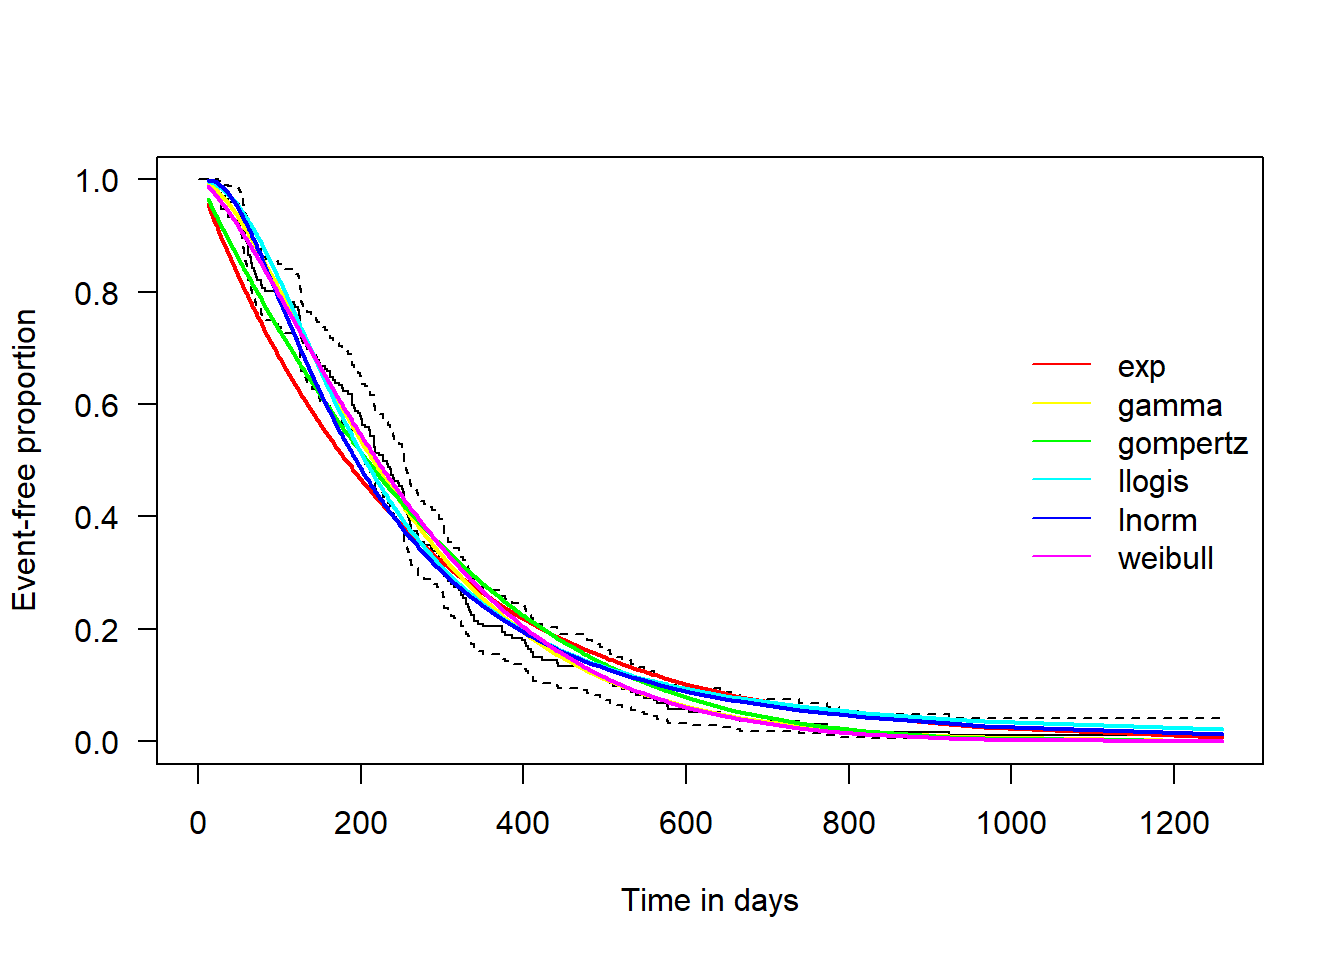
\includegraphics{Markov_3state_files/figure-latex/unnamed-chunk-11-1.pdf}

\begin{Shaded}
\begin{Highlighting}[]
\CommentTok{\# The vertical line shows you when your sick (OS) population is the greatest that it will ever be, but it can be changed from which.max to other things (so it is finding which cycle the proportion sick is the highest and putting a vertical line there).}



\CommentTok{\# So, you can see in the graph everyone starts in the PFS state, but that this falls over time as people progress and leave this state, then you see OS start to peak up but then fall again as people leave this state to go into the dead state, which is an absorbing state and by the end will include everyone.}
\end{Highlighting}
\end{Shaded}

\hypertarget{overall-survival-os}{%
\subsection{06.2 Overall Survival (OS)}\label{overall-survival-os}}

Although in the context of my analysis this would be PFS + OS because it
is drawn from the DARTH model where healthy and sick make up OS, while
dead means not OS (obviously).

\begin{Shaded}
\begin{Highlighting}[]
\NormalTok{v\_os }\OtherTok{\textless{}{-}} \DecValTok{1} \SpecialCharTok{{-}}\NormalTok{ m\_M\_SoC[, }\StringTok{"Dead"}\NormalTok{]    }\CommentTok{\# calculate the overall survival (OS) probability}
\NormalTok{v\_os }\OtherTok{\textless{}{-}} \FunctionTok{rowSums}\NormalTok{(m\_M\_SoC[, }\DecValTok{1}\SpecialCharTok{:}\DecValTok{2}\NormalTok{])  }\CommentTok{\# alternative way of calculating the OS probability}

\CommentTok{\# I could do my own version of this and chose just to look at pfs, rather than column 1 and 2 to look at anyone not dead.}

\CommentTok{\# i.e. v\_os \textless{}{-} (m\_M\_SoC[, 1])}

\CommentTok{\# best practice would be to rename v\_os if I am looking at something that isnt os, i.e. v\_pfs and to of course update the table legend, bearing in mind that yet again this is all for standard of care, and that if I wanted to know this for treatment a and/or treatment b I would need to replace the Markov model matrix above.}


\FunctionTok{plot}\NormalTok{(v\_os, }\AttributeTok{type =} \StringTok{\textquotesingle{}l\textquotesingle{}}\NormalTok{, }
     \AttributeTok{ylim =} \FunctionTok{c}\NormalTok{(}\DecValTok{0}\NormalTok{, }\DecValTok{1}\NormalTok{),}
     \AttributeTok{ylab =} \StringTok{"Survival probability"}\NormalTok{,}
     \AttributeTok{xlab =} \StringTok{"Cycle"}\NormalTok{,}
     \AttributeTok{main =} \StringTok{"Overall Survival"}\NormalTok{)  }\CommentTok{\# create a simple plot showing the OS}

\CommentTok{\# add grid }
\FunctionTok{grid}\NormalTok{(}\AttributeTok{nx =}\NormalTok{ n\_cycles, }\AttributeTok{ny =} \DecValTok{10}\NormalTok{, }\AttributeTok{col =} \StringTok{"lightgray"}\NormalTok{, }\AttributeTok{lty =} \StringTok{"dotted"}\NormalTok{, }\AttributeTok{lwd =} \FunctionTok{par}\NormalTok{(}\StringTok{"lwd"}\NormalTok{), }
     \AttributeTok{equilogs =} \ConstantTok{TRUE}\NormalTok{) }
\end{Highlighting}
\end{Shaded}

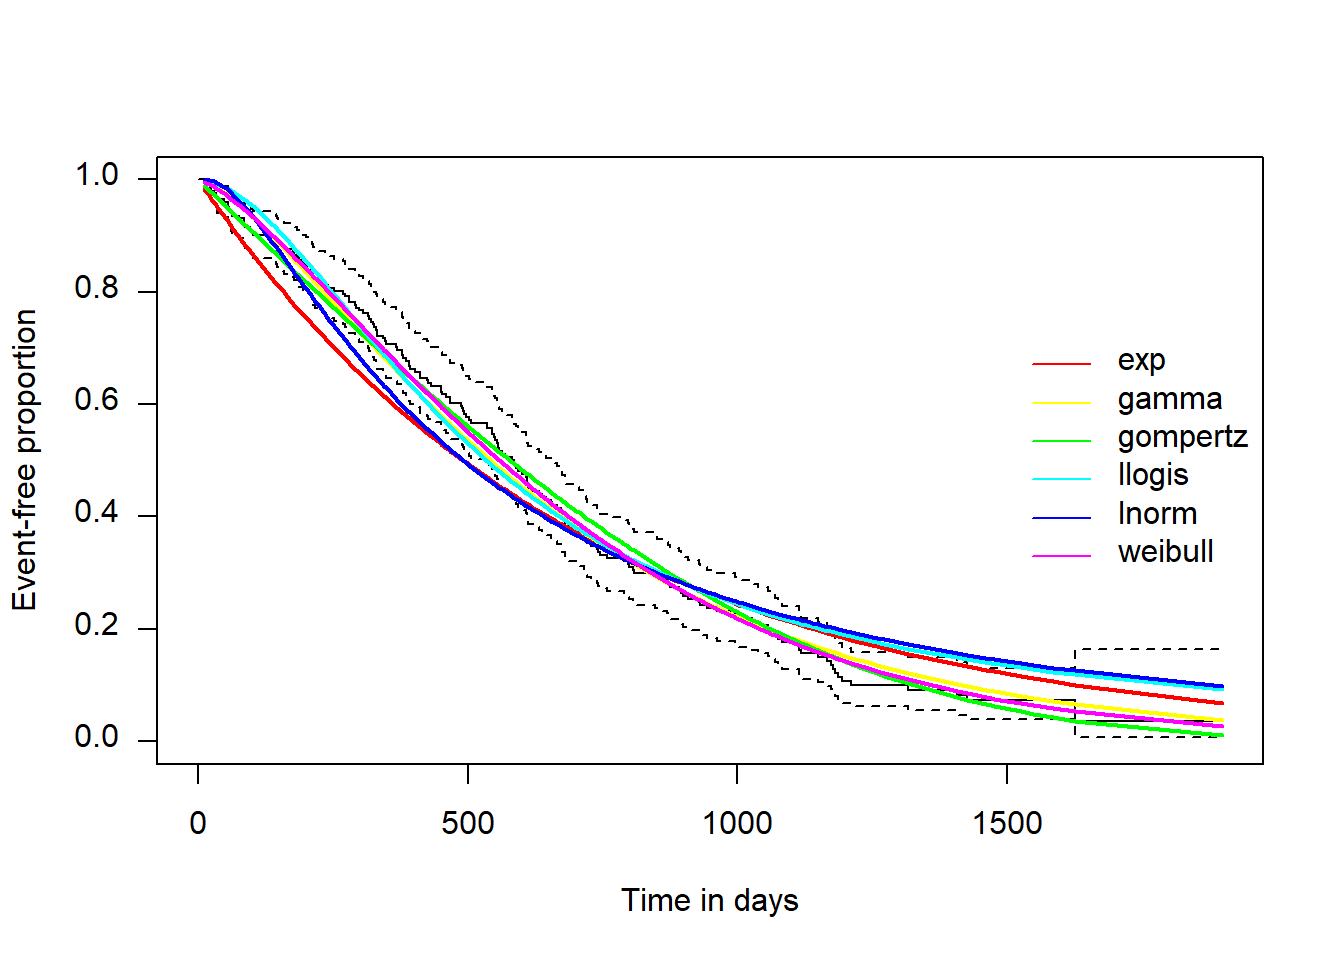
\includegraphics{Markov_3state_files/figure-latex/unnamed-chunk-12-1.pdf}

\begin{Shaded}
\begin{Highlighting}[]
\CommentTok{\# Per 1:12 hour mark of: C:\textbackslash{}Users\textbackslash{}Jonathan\textbackslash{}OneDrive {-} Royal College of Surgeons in Ireland\textbackslash{}COLOSSUS\textbackslash{}Training Resources\textbackslash{}Cost{-}Effectiveness and Decision Modeling using R Workshop \textbackslash{}\_ DARTH\textbackslash{}August\textbackslash{}\_25\textbackslash{}Live Session Recording\textbackslash{}Live Session Recording August 25th WITH CHAT.mkv}

\CommentTok{\# Often you have a survival curve as input to your model [I guess from a published study], and having that survival curve you need to parameterise your model so that you match that survival curve, and that would be a process of, potentially of calibration, if you can\textquotesingle{}t use the parameters directly in your model.}

\CommentTok{\# So, you could produce your survival curve and compare it to curves from trials, etc., to calibrate your model. So. we\textquotesingle{}ll probably do this and have it in an appendix section.}

\CommentTok{\# For calibration purposes, you want to make sure that your model is outputting something that\textquotesingle{}s comparable to the publications out there on actual data on the same type of patients.}

\CommentTok{\# Part of being comparable to the real world is that if there is a censoring process in actual patient data, then you could incorporate this process into the model to reflect that in your model and to ensure that your own model is comparable to the existing models which may be losing people due to censoring, etc., and which you\textquotesingle{}ll then need to incorporate into your model to be comparable. }


\CommentTok{\# Another interesting thing you can do is, plot this to ask is that reasonable, does that make sense that this many people are alive after this amount of time? Is the OS what I would expect it to be?}
\end{Highlighting}
\end{Shaded}

\hypertarget{life-expectancy-le}{%
\subsection{06.2.1 Life Expectancy (LE)}\label{life-expectancy-le}}

\begin{Shaded}
\begin{Highlighting}[]
\NormalTok{v\_le }\OtherTok{\textless{}{-}} \FunctionTok{sum}\NormalTok{(v\_os)  }\CommentTok{\# summing probability of OS over time  (i.e. life expectancy)}

\CommentTok{\# Basically we are summing all the alive states over time through over all the cycles, so }

\CommentTok{\# v\_os \textless{}{-} rowSums(m\_M\_SoC[, 1:2])}

\CommentTok{\# Is basically the PFS and OS added together.}

\CommentTok{\# Also bear in mind that this is life expectancy under standard of care, and not under either of the new treatments, per: \# v\_os \textless{}{-} rowSums(m\_M\_SoC[, 1:2]) above.}

\NormalTok{v\_le}
\end{Highlighting}
\end{Shaded}

\begin{verbatim}
## [1] 24.26038
\end{verbatim}

\begin{Shaded}
\begin{Highlighting}[]
\CommentTok{\# So, this gives a value of [1] 24.26038, that is [1] 24.26038 cycles, where in the context of our model, cycles are months, so the life expectancy for our population of patients is 24 months.}


\CommentTok{\# Discounted life expectancy:}

\CommentTok{\# If you wanted discounted life expectancy, if you were using life years and you wanted them discounted for your health economic outcomes, you could apply the discount rates {-} the discount factors {-} to the vector for overall survival [v\_os] and then take it\textquotesingle{}s sum [add it up] as above to get life expectancy that is discounted.}

\CommentTok{\# As the 1:12 hour mark of: C:\textbackslash{}Users\textbackslash{}Jonathan\textbackslash{}OneDrive {-} Royal College of Surgeons in Ireland\textbackslash{}COLOSSUS\textbackslash{}Training Resources\textbackslash{}Cost{-}Effectiveness and Decision Modeling using R Workshop \_ DARTH\textbackslash{}August\_25\textbackslash{}Live Session Recording\textbackslash{}Live Session Recording August 25th WITH CHAT.mkv}
\end{Highlighting}
\end{Shaded}

\hypertarget{disease-prevalence}{%
\subsection{06.3 Disease prevalence}\label{disease-prevalence}}

\begin{Shaded}
\begin{Highlighting}[]
\CommentTok{\# Disease prevalence is the proportion who are sick divided by the proportion who are alive, so it\textquotesingle{}s necessary to account for the fact that some of the cohort have died, so you only calculate prevalence among people who are alive,in the diagram you can see it plateauing over time, even though the number of people in the OS (or "progressed") state have gone up and come down over time and this is because this is prevalence as a proportion of those who are alive, and there are few people who are still alive by cycle 60.}

\CommentTok{\# Probably looks a bit funny dividing OS by v\_os below, but it\textquotesingle{}s necessary to remember that v\_os is PFS + OS.}

\CommentTok{\# So, I guess in our context you can think of this as progression prevalence over time:}

\NormalTok{v\_prev }\OtherTok{\textless{}{-}}\NormalTok{ m\_M\_SoC[, }\StringTok{"OS"}\NormalTok{]}\SpecialCharTok{/}\NormalTok{v\_os}
\FunctionTok{plot}\NormalTok{(v\_prev,}
     \AttributeTok{ylim =} \FunctionTok{c}\NormalTok{(}\DecValTok{0}\NormalTok{, }\DecValTok{1}\NormalTok{),}
     \AttributeTok{ylab =} \StringTok{"Prevalence"}\NormalTok{,}
     \AttributeTok{xlab =} \StringTok{"Cycle"}\NormalTok{,}
     \AttributeTok{main =} \StringTok{"Disease prevalence"}\NormalTok{)}
\end{Highlighting}
\end{Shaded}

\includegraphics{Markov_3state_files/figure-latex/unnamed-chunk-14-1.pdf}

\hypertarget{compute-cost-effectiveness-outcomes}{%
\section{07 Compute Cost-Effectiveness
Outcomes}\label{compute-cost-effectiveness-outcomes}}

\hypertarget{mean-costs-and-qalys-for-each-strategy}{%
\subsection{07.1 Mean Costs and QALYs for each
strategy}\label{mean-costs-and-qalys-for-each-strategy}}

\begin{Shaded}
\begin{Highlighting}[]
\CommentTok{\# per cycle}
\CommentTok{\# calculate expected costs by multiplying cohort trace with the cost vector for the different health states}

\CommentTok{\# Basically, you take the cohort trace over time for each strategy [m\_M\_SoC] and multiply this by a vector of our costs for each state: [c(c\_H, c\_S, c\_D)] {-}\textgreater{} So, basically the number of people in each state at each cycle multiplied by the cost of being in that state [cost of healthy, cost of sick and cost of dead] for each strategy that we look at (standard of care, treatment A and treatment B).}

\CommentTok{\# Bear in mind we are doing matrix multiplication [\%*\%], because what this does is for each cycle [row in the matrix], take the vector of costs, and multiply it be the distribution in that cycle [breakdown of proportions in the states in that row] and add it all together, to get the total costs for that cycle [row]. This gives us a vector of the costs accrued in this cohort of individuals ending up in these different states for each cycle on a per person basis, because it\textquotesingle{}s a cohort distribution (it always sums to 1).}

\CommentTok{\# So, in cycle 1 everyone is in the OS state, so they only incur the OS cost, as more and more time passes and more and more people get sick, the costs increases due to more people being in the PFS state, but over time this falls again as more and more people go into the dead state, which has no costs as we don\textquotesingle{}t treat corpses.}

\NormalTok{v\_tc\_SoC  }\OtherTok{\textless{}{-}}\NormalTok{ m\_M\_SoC  }\SpecialCharTok{\%*\%} \FunctionTok{c}\NormalTok{(c\_H, c\_S, c\_D)  }
\NormalTok{v\_tc\_trtA }\OtherTok{\textless{}{-}}\NormalTok{ m\_M\_trtA }\SpecialCharTok{\%*\%} \FunctionTok{c}\NormalTok{(c\_H }\SpecialCharTok{+}\NormalTok{ c\_trtA, c\_S, c\_D)  }
\NormalTok{v\_tc\_trtB }\OtherTok{\textless{}{-}}\NormalTok{ m\_M\_trtB }\SpecialCharTok{\%*\%} \FunctionTok{c}\NormalTok{(c\_H }\SpecialCharTok{+}\NormalTok{ c\_trtB, c\_S, c\_D)  }

\CommentTok{\# calculate expected QALYs by multiplying cohort trace with the utilities for the different health states }

\CommentTok{\# The three vectors of utilities are basically built in the exact same way as the three vectors of costs above:}

\NormalTok{v\_tu\_SoC  }\OtherTok{\textless{}{-}}\NormalTok{ m\_M\_SoC  }\SpecialCharTok{\%*\%} \FunctionTok{c}\NormalTok{(u\_H, u\_S, u\_D)  }
\NormalTok{v\_tu\_trtA }\OtherTok{\textless{}{-}}\NormalTok{ m\_M\_trtA }\SpecialCharTok{\%*\%} \FunctionTok{c}\NormalTok{(u\_H, u\_S, u\_D) }
\NormalTok{v\_tu\_trtB }\OtherTok{\textless{}{-}}\NormalTok{ m\_M\_trtB }\SpecialCharTok{\%*\%} \FunctionTok{c}\NormalTok{(u\_H, u\_S, u\_D) }

\CommentTok{\# These are quality adjusted cycles, these are quality adjusted life years where cycles are annual, so I need to consider what this means for utility where cycles are monthly... I suppose it\textquotesingle{}s just quality adjusted monthly utility.}

\CommentTok{\# You can see above that there are no utility differences between the different treatments considered: c(u\_H, u\_S, u\_D), it\textquotesingle{}s just different utilities per the health states people are in.}

\CommentTok{\# If we did want to do different utilities for the health state you are in per the treatment you are on, we could define this in the input parameters and then add this in above when creating the vector of utilities for that treatment.}
\end{Highlighting}
\end{Shaded}

\begin{Shaded}
\begin{Highlighting}[]
\CommentTok{\# There\textquotesingle{}s probably a more elegant way to do this, but if I wanted to add in the once off cost of the COSLOSSUS test, I could do something like the below:}

\CommentTok{\# v\_tc\_trtA \textless{}{-}  v\_tc\_trtA+10}
\CommentTok{\# v\_tc\_trtB \textless{}{-}  v\_tc\_trtB+100}

\CommentTok{\# I just need to think about this and does it make sense, because it\textquotesingle{}s adding to the cost each cycle, so probably the best indicator would be whether the cost outputted in 07.2 is only higher by the cost of the test when we do this, or if it is higher by a number of other costs, so I can check that below when adding costs in.}
\end{Highlighting}
\end{Shaded}

\hypertarget{discounted-mean-costs-and-qalys}{%
\subsection{07.2 Discounted Mean Costs and
QALYs}\label{discounted-mean-costs-and-qalys}}

\begin{Shaded}
\begin{Highlighting}[]
\CommentTok{\# Finally, we\textquotesingle{}ll aggregate these costs and utilities into overall discounted mean (average) costs and utilities.}

\CommentTok{\# So, we take the vector of costs, transposing it [the t() bit] to make it a 1 row matrix and using matrix multiplication [\%*\%] to multiply it by that discount factor vector, which is what you multiply by the outcome in each cycle to get the discounted value of the outcome for that cycle, and then it will all be summed all together across all cycles [across all cells of the 1 row matrix]. Giving you tc\_d\_SoC which is a scalar, or a single value, which is the lifetime expected cost for an average person under standard of care in this cohort. }


\CommentTok{\# Discount costs by multiplying the cost vector with discount weights (v\_dwc) }
\NormalTok{tc\_d\_SoC  }\OtherTok{\textless{}{-}}  \FunctionTok{t}\NormalTok{(v\_tc\_SoC)  }\SpecialCharTok{\%*\%}\NormalTok{ v\_dwc}
\NormalTok{tc\_d\_trtA }\OtherTok{\textless{}{-}}  \FunctionTok{t}\NormalTok{(v\_tc\_trtA) }\SpecialCharTok{\%*\%}\NormalTok{ v\_dwc}
\NormalTok{tc\_d\_trtB }\OtherTok{\textless{}{-}}  \FunctionTok{t}\NormalTok{(v\_tc\_trtB) }\SpecialCharTok{\%*\%}\NormalTok{ v\_dwc}


\CommentTok{\# So, now we have the average cost per person for treatment with standard of care, treatment A and treatment B. }


\CommentTok{\# Discount QALYS by multiplying the QALYs vector with discount weights (v\_dwe) [probably utilities would be a better term here, as it\textquotesingle{}s monthly health state quality of life, rather than yearly health state quality of life]}
\NormalTok{tu\_d\_SoC  }\OtherTok{\textless{}{-}}  \FunctionTok{t}\NormalTok{(v\_tu\_SoC)  }\SpecialCharTok{\%*\%}\NormalTok{ v\_dwe}
\NormalTok{tu\_d\_trtA }\OtherTok{\textless{}{-}}  \FunctionTok{t}\NormalTok{(v\_tu\_trtA) }\SpecialCharTok{\%*\%}\NormalTok{ v\_dwe}
\NormalTok{tu\_d\_trtB }\OtherTok{\textless{}{-}}  \FunctionTok{t}\NormalTok{(v\_tu\_trtB) }\SpecialCharTok{\%*\%}\NormalTok{ v\_dwe}

\CommentTok{\# Store them into a vector {-}\textgreater{} So, we\textquotesingle{}ll take the single values for cost for an average person under standard of care, treatment A and treatment B, and stored them in a vector v\_tc\_d}
\NormalTok{v\_tc\_d }\OtherTok{\textless{}{-}} \FunctionTok{c}\NormalTok{(tc\_d\_SoC, tc\_d\_trtA, tc\_d\_trtB)}
\NormalTok{v\_tu\_d }\OtherTok{\textless{}{-}} \FunctionTok{c}\NormalTok{(tu\_d\_SoC, tu\_d\_trtA, tu\_d\_trtB)}

\NormalTok{v\_tc\_d}
\end{Highlighting}
\end{Shaded}

\begin{verbatim}
## [1]  8915.034 19280.793 34371.418
\end{verbatim}

\begin{Shaded}
\begin{Highlighting}[]
\NormalTok{v\_tu\_d}
\end{Highlighting}
\end{Shaded}

\begin{verbatim}
## [1] 13.62825 14.77798 18.02450
\end{verbatim}

\begin{Shaded}
\begin{Highlighting}[]
\CommentTok{\# To make things a little easier to read we might name these values what they are costs for, so we can use the vector of strategy names [v\_names\_str] to name the values:}

\FunctionTok{names}\NormalTok{ (v\_tc\_d) }\OtherTok{\textless{}{-}}\NormalTok{ v\_names\_str}
\NormalTok{v\_tc\_d}
\end{Highlighting}
\end{Shaded}

\begin{verbatim}
## Standard of Care        EPI Assay        HDX Assay 
##         8915.034        19280.793        34371.418
\end{verbatim}

\begin{Shaded}
\begin{Highlighting}[]
\FunctionTok{names}\NormalTok{ (v\_tu\_d) }\OtherTok{\textless{}{-}}\NormalTok{ v\_names\_str}
\NormalTok{v\_tu\_d}
\end{Highlighting}
\end{Shaded}

\begin{verbatim}
## Standard of Care        EPI Assay        HDX Assay 
##         13.62825         14.77798         18.02450
\end{verbatim}

\begin{Shaded}
\begin{Highlighting}[]
\CommentTok{\# For utility, the utility values aren\textquotesingle{}t different for the different states depending on the treatment strategy, i.e. SOC, Treatment A and Treatment B, but the time spent in the states with the associated utility is different due to the treatment you\textquotesingle{}re on, so your utility value will be higher if the treatment keeps you well for longer so that you stay in a higher utility state for longer than a lower utility state, i.e., progression.}


\CommentTok{\# Dataframe with discounted costs and effectiveness}

\CommentTok{\# So then we aggregate them into a dataframe with our discounted costs and utilities, and then we use this to calculate ICERs in: \#\# 07.3 Compute ICERs of the Markov model}

\NormalTok{df\_ce }\OtherTok{\textless{}{-}} \FunctionTok{data.frame}\NormalTok{(}\AttributeTok{Strategy =}\NormalTok{ v\_names\_str,}
                    \AttributeTok{Cost     =}\NormalTok{ v\_tc\_d, }
                    \AttributeTok{Effect   =}\NormalTok{ v\_tu\_d)}
\NormalTok{df\_ce}
\end{Highlighting}
\end{Shaded}

\begin{verbatim}
##                          Strategy      Cost   Effect
## Standard of Care Standard of Care  8915.034 13.62825
## EPI Assay               EPI Assay 19280.793 14.77798
## HDX Assay               HDX Assay 34371.418 18.02450
\end{verbatim}

\hypertarget{compute-icers-of-the-markov-model}{%
\subsection{07.3 Compute ICERs of the Markov
model}\label{compute-icers-of-the-markov-model}}

(If I wanted to take a Net Monetary Benefit (NMB) approach instead, I
could go to the 35 minute mark of: C:\Users\Jonathan\OneDrive - Royal
College of Surgeons in
Ireland\COLOSSUS\Training Resources\Cost-Effectiveness and Decision
Modeling using R Workshop \_ DARTH\August\_24\Live Session
Recording\Live Session Recording August 24th.mp4)

\begin{Shaded}
\begin{Highlighting}[]
\NormalTok{df\_cea }\OtherTok{\textless{}{-}} \FunctionTok{calculate\_icers}\NormalTok{(}\AttributeTok{cost       =}\NormalTok{ df\_ce}\SpecialCharTok{$}\NormalTok{Cost,}
                          \AttributeTok{effect     =}\NormalTok{ df\_ce}\SpecialCharTok{$}\NormalTok{Effect,}
                          \AttributeTok{strategies =}\NormalTok{ df\_ce}\SpecialCharTok{$}\NormalTok{Strategy}
\NormalTok{                          )}
\NormalTok{df\_cea}
\end{Highlighting}
\end{Shaded}

\begin{verbatim}
##           Strategy      Cost   Effect Inc_Cost Inc_Effect     ICER Status
## 1 Standard of Care  8915.034 13.62825       NA         NA       NA     ND
## 2        HDX Assay 34371.418 18.02450 25456.38   4.396243 5790.485     ND
## 3        EPI Assay 19280.793 14.77798       NA         NA       NA     ED
\end{verbatim}

\begin{Shaded}
\begin{Highlighting}[]
\CommentTok{\# The above uses the DARTHtools package to calculate our ICERS, incremental cost and incremental effectiveness, and also describes dominance status:}

\CommentTok{\# This uses the "calculate\_icers function", which does all the sorting, all the prioritization, and then computes the dominance, and not dominance, etc., and there\textquotesingle{}s a publication on the methods behind this, based on a method from colleagues in Stanford.}

\CommentTok{\# The default view is ordered by dominance status (ND = non{-}dominated, ED = extended/weak dominance, or D= strong dominance), and then ascending by cost per: https://cran.r{-}project.org/web/packages/dampack/vignettes/basic\_cea.html}


\CommentTok{\# The icer object can be easily formatted into a publication quality table using the kableExtra package.}

\CommentTok{\# library(kableExtra)}
\CommentTok{\# library(dplyr)}
\CommentTok{\# df\_cea \%\textgreater{}\%}
\CommentTok{\#  kable() \%\textgreater{}\%}
\CommentTok{\#  kable\_styling()}
\end{Highlighting}
\end{Shaded}

\hypertarget{plot-frontier-of-the-markov-model}{%
\subsection{07.4 Plot frontier of the Markov
model}\label{plot-frontier-of-the-markov-model}}

\begin{Shaded}
\begin{Highlighting}[]
\FunctionTok{plot}\NormalTok{(df\_cea, }\AttributeTok{effect\_units =} \StringTok{"QALYs"}\NormalTok{, }\AttributeTok{label =} \StringTok{"all"}\NormalTok{)}
\end{Highlighting}
\end{Shaded}

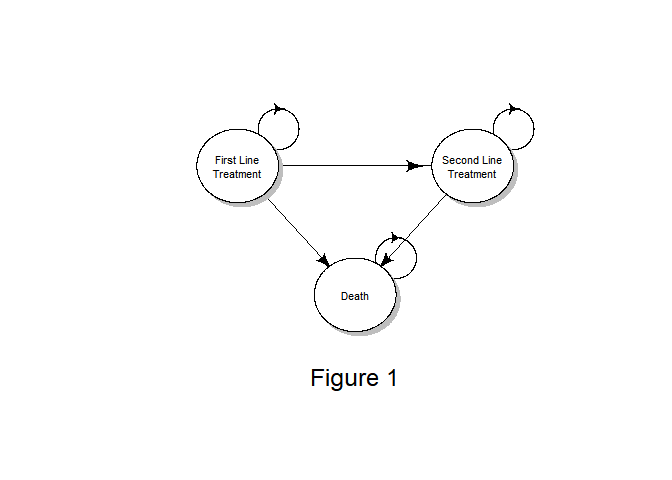
\includegraphics{Markov_3state_files/figure-latex/unnamed-chunk-19-1.pdf}

\begin{Shaded}
\begin{Highlighting}[]
\CommentTok{\# When we plot it we have 3 strategies it is possible that something would be off the frontier, would be weakly dominated or strongly dominated, with just a few strategies it\textquotesingle{}s not necessarily that impressive, but with lots of strategies then dampack can be helpful.}
\end{Highlighting}
\end{Shaded}

The bottom axis of the above diagram shows you how effective the
intervention is, the y axis shows you how costly the intervention is,
here standard of care is cheaper but less effective than treatment B,
which is more effective but more expensive, treatment A is not on the
frontier, it has been dominated.

(If I wanted to see an example where the frontier doesnt exist, I could
go to the 38 minute mark of: C:\Users\Jonathan\OneDrive - Royal College
of Surgeons in Ireland\COLOSSUS\Training Resources\Cost-Effectiveness
and Decision Modeling using R Workshop \_ DARTH\August\_24\Live Session
Recording\Live Session Recording August 24th.mp4)

\url{https://www.google.ie/search?q=icer+fronter\&hl=en\&dcr=0\&ei=nerzYYS_AciHhbIPlqyMuAk\&ved=0ahUKEwjEgar1wdT1AhXIQ0EAHRYWA5cQ4dUDCA4\&uact=5\&oq=icer+fronter\&gs_lcp=Cgdnd3Mtd2l6EAMyBwghEAoQoAE6BwgAEEcQsAM6BQgAEJECOgsIABCABBCxAxCDAToOCC4QgAQQsQMQxwEQowI6CwguELEDEMcBEK8BOg4ILhCABBCxAxDHARDRAzoICAAQsQMQgwE6BQguEJECOgQIABBDOgcIABCxAxBDOggIABCABBCxAzoOCC4QgAQQsQMQxwEQrwE6CAguEIAEELEDOgcIABDJAxBDOgUIABCSAzoFCAAQgAQ6CwguEIAEEMcBENEDOgUILhCABDoLCC4QgAQQxwEQrwE6BAgAEAo6CgguEMcBENEDEAo6BAguEAo6BwgAEMkDEAo6BggAEBYQHjoICAAQFhAKEB46BAgAEA06BQghEKABSgQIQRgASgQIRhgAUKIJWJYZYNEbaANwAngAgAGMAYgB6AiSAQM4LjSYAQCgAQHIAQjAAQE\&sclient=gws-wiz}

\url{https://yhec.co.uk/glossary/cost-effectiveness-frontier/}

\href{https://www.hiqa.ie/sites/default/files/2017-01/Revised_Economic_Guidelines_posted_100714.pdf}{\textless https://www.hiqa.ie/sites/default/files/2017-01/Revised\_Economic\_Guidelines\_posted\_100714.pdf\textgreater{}}
{[}also saved here:
C:\textbackslash Users\textbackslash Jonathan\textbackslash OneDrive -
Royal College of Surgeons in
Ireland\textbackslash COLOSSUS\textbackslash R
Code\textbackslash GitHub\textbackslash COLOSSUS\_Model\textbackslash Revised\_Economic\_Guidelines\_posted\_100714.pdf{]}

\url{https://researchonline.lshtm.ac.uk/id/eprint/4648686/1/The\%20efficiency-frontier\%20approach\%20for\%20health_GREEN\%20AAM.pdf}
also saved here:C:\Users\Jonathan\OneDrive - Royal College of Surgeons
in
Ireland\COLOSSUS\R Code\GitHub\COLOSSUS\_Model\The efficiency-frontier
approach for health\_GREEN AAM.pdf

The efficiency frontier is described on page 277 {[}in the textbook{]}
of:
\url{file:///C:/Users/Jonathan/OneDrive\%20-\%20Royal\%20College\%20of\%20Surgeons\%20in\%20Ireland/COLOSSUS/R\%20Code/GitHub/COLOSSUS_Model/(Cambridge\%20medicine)\%20Hunink,\%20M.\%20G.\%20Myriam_Weinstein,\%20Milton\%20C\%20-\%20Decision\%20making\%20in\%20health\%20and\%20medicine_\%20integrating\%20evidence\%20and\%20values.pdf}

\hypertarget{sensitivity-analysis-below}{%
\section{\texorpdfstring{\textbf{Sensitivity Analysis
Below:}}{Sensitivity Analysis Below:}}\label{sensitivity-analysis-below}}

I've put detailed notes in:

C:\Users\Jonathan\OneDrive - Royal College of Surgeons in
Ireland\COLOSSUS\Training Resources\Cost-Effectiveness and Decision
Modeling using R Workshop \_
DARTH\August\_27\textbackslash3\_SA\_material\markov\_sick-sicker\_SA\_solutions

Which should be read in tangent with: C:\Users\Jonathan\OneDrive - Royal
College of Surgeons in
Ireland\COLOSSUS\Training Resources\Decision Modelling - Advanced
Course\A2\_Making Models Probabilistic\A2.1.2 Distributions for
parameters\notes.txt

when doing the sensitivity analysis below:

There is similarly relevant information at the 1:38 hour mark of:
C:\Users\Jonathan\OneDrive - Royal College of Surgeons in
Ireland\COLOSSUS\Training Resources\Cost-Effectiveness and Decision
Modeling using R Workshop \_ DARTH\August\_25\Live Session
Recording\Live Session Recording August 25th WITH CHAT.mkv

And in this document:

C:\textbackslash Users\textbackslash Jonathan\textbackslash OneDrive -
Royal College of Surgeons in
Ireland\textbackslash COLOSSUS\textbackslash Briggs et al 2012 model
parameter estimation and uncertainty.pdf

\hypertarget{deterministic-sensitivity-analysis}{%
\section{08 Deterministic Sensitivity
Analysis}\label{deterministic-sensitivity-analysis}}

\hypertarget{list-of-input-parameters}{%
\subsection{08.1 List of input
parameters}\label{list-of-input-parameters}}

Create list \texttt{l\_params\_all} with all input probabilities, cost
and utilities.

\begin{Shaded}
\begin{Highlighting}[]
\NormalTok{l\_params\_all }\OtherTok{\textless{}{-}} \FunctionTok{as.list}\NormalTok{(}\FunctionTok{data.frame}\NormalTok{(}
  \AttributeTok{p\_HD      =} \FloatTok{0.01}\NormalTok{,  }\CommentTok{\# probability of dying when OS}
  \AttributeTok{p\_HS\_SoC  =} \FloatTok{0.05}\NormalTok{,  }\CommentTok{\# probability of becoming PFS when OS, under standard of care}
  \AttributeTok{p\_HS\_trtA =} \FloatTok{0.04}\NormalTok{,  }\CommentTok{\# probability of becoming PFS when OS, under treatment A}
  \AttributeTok{p\_HS\_trtB =} \FloatTok{0.02}\NormalTok{,  }\CommentTok{\# probability of becoming PFS when OS, under treatment B}
  \AttributeTok{p\_SD      =} \FloatTok{0.1}\NormalTok{,   }\CommentTok{\# probability of dying when PFS}
  \AttributeTok{c\_H       =} \DecValTok{400}\NormalTok{,   }\CommentTok{\# cost of one cycle in OS state}
  \AttributeTok{c\_S       =} \DecValTok{1000}\NormalTok{,  }\CommentTok{\# cost of one cycle in PFS state}
  \AttributeTok{c\_D       =} \DecValTok{0}\NormalTok{,     }\CommentTok{\# cost of one cycle in dead state}
  \AttributeTok{c\_trtA    =} \DecValTok{800}\NormalTok{,   }\CommentTok{\# cost of treatment A (per cycle)}
  \AttributeTok{c\_trtB    =} \DecValTok{1500}\NormalTok{,  }\CommentTok{\# cost of treatment B (per cycle)}
  \AttributeTok{u\_H       =} \DecValTok{1}\NormalTok{,     }\CommentTok{\# utility when OS }
  \AttributeTok{u\_S       =} \FloatTok{0.5}\NormalTok{,   }\CommentTok{\# utility when PFS}
  \AttributeTok{u\_D       =} \DecValTok{0}\NormalTok{,     }\CommentTok{\# utility when dead}
  \AttributeTok{d\_e       =} \FloatTok{0.03}\NormalTok{,  }\CommentTok{\# discount factor for effectiveness}
  \AttributeTok{d\_c       =} \FloatTok{0.03}   \CommentTok{\# discount factor for costs}
\NormalTok{))}

\CommentTok{\# store the parameter names into a vector}
\NormalTok{v\_names\_params }\OtherTok{\textless{}{-}} \FunctionTok{names}\NormalTok{(l\_params\_all)}
\end{Highlighting}
\end{Shaded}

\hypertarget{load-pfs-pfser-markov-model-function}{%
\subsection{08.2 Load PFS-PFSer Markov model
function}\label{load-pfs-pfser-markov-model-function}}

To make the function work for my health states I rename ``health'' and
``sick'' in it to ``PFS'' and ``OS'' respectively.

\begin{Shaded}
\begin{Highlighting}[]
\FunctionTok{source}\NormalTok{(}\StringTok{"Functions\_markov\_3state.R"}\NormalTok{)}
\CommentTok{\# Test function}
\FunctionTok{calculate\_ce\_out}\NormalTok{(l\_params\_all)}
\end{Highlighting}
\end{Shaded}

\begin{verbatim}
##           Strategy      Cost   Effect      NMB
## 1 Standard of Care  8915.034 13.62825 127367.5
## 2        EPI Assay 19280.793 14.77798 128499.0
## 3        HDX Assay 34371.418 18.02450 145873.5
\end{verbatim}

\hypertarget{one-way-sensitivity-analysis-owsa}{%
\subsection{08.3 One-way sensitivity analysis
(OWSA)}\label{one-way-sensitivity-analysis-owsa}}

\begin{Shaded}
\begin{Highlighting}[]
\FunctionTok{options}\NormalTok{(}\AttributeTok{scipen =} \DecValTok{999}\NormalTok{) }\CommentTok{\# disabling scientific notation in R}
\CommentTok{\# dataframe containing all parameters, their base case values, and the min and }
\CommentTok{\# max values of the parameters of interest }
\NormalTok{df\_params\_owsa }\OtherTok{\textless{}{-}} \FunctionTok{data.frame}\NormalTok{(}\AttributeTok{pars =} \FunctionTok{c}\NormalTok{(}\StringTok{"c\_trtA"}\NormalTok{, }\StringTok{"c\_trtB"}\NormalTok{, }\StringTok{"c\_S"}\NormalTok{),}
                             \AttributeTok{min  =} \FunctionTok{c}\NormalTok{(}\DecValTok{300}\NormalTok{ , }\DecValTok{500}\NormalTok{, }\DecValTok{500}\NormalTok{),  }\CommentTok{\# min parameter values}
                             \AttributeTok{max  =} \FunctionTok{c}\NormalTok{(}\DecValTok{1200}\NormalTok{, }\DecValTok{2000}\NormalTok{, }\DecValTok{2000}\NormalTok{)  }\CommentTok{\# max parameter values}
\NormalTok{)}

\NormalTok{owsa\_nmb  }\OtherTok{\textless{}{-}} \FunctionTok{run\_owsa\_det}\NormalTok{(}\AttributeTok{params\_range     =}\NormalTok{ df\_params\_owsa,    }\CommentTok{\# dataframe with parameters for OWSA}
                          \AttributeTok{params\_basecase  =}\NormalTok{ l\_params\_all,      }\CommentTok{\# list with all parameters}
                          \AttributeTok{nsamp            =} \DecValTok{100}\NormalTok{,               }\CommentTok{\# number of parameter values}
                          \AttributeTok{FUN              =}\NormalTok{ calculate\_ce\_out,  }\CommentTok{\# function to compute outputs}
                          \AttributeTok{outcomes         =} \FunctionTok{c}\NormalTok{(}\StringTok{"NMB"}\NormalTok{),          }\CommentTok{\# output to do the OWSA on}
                          \AttributeTok{strategies       =}\NormalTok{ v\_names\_str,       }\CommentTok{\# names of the strategies}
                          \AttributeTok{n\_wtp            =} \DecValTok{5000}\NormalTok{)              }\CommentTok{\# extra argument to pass to FUN}
\end{Highlighting}
\end{Shaded}

\begin{verbatim}
##   |                                                                              |                                                                      |   0%  |                                                                              |                                                                      |   1%  |                                                                              |=                                                                     |   1%  |                                                                              |=                                                                     |   2%  |                                                                              |==                                                                    |   2%  |                                                                              |==                                                                    |   3%  |                                                                              |===                                                                   |   4%  |                                                                              |===                                                                   |   5%  |                                                                              |====                                                                  |   5%  |                                                                              |====                                                                  |   6%  |                                                                              |=====                                                                 |   7%  |                                                                              |=====                                                                 |   8%  |                                                                              |======                                                                |   8%  |                                                                              |======                                                                |   9%  |                                                                              |=======                                                               |   9%  |                                                                              |=======                                                               |  10%  |                                                                              |=======                                                               |  11%  |                                                                              |========                                                              |  11%  |                                                                              |========                                                              |  12%  |                                                                              |=========                                                             |  12%  |                                                                              |=========                                                             |  13%  |                                                                              |==========                                                            |  14%  |                                                                              |==========                                                            |  15%  |                                                                              |===========                                                           |  15%  |                                                                              |===========                                                           |  16%  |                                                                              |============                                                          |  17%  |                                                                              |============                                                          |  18%  |                                                                              |=============                                                         |  18%  |                                                                              |=============                                                         |  19%  |                                                                              |==============                                                        |  19%  |                                                                              |==============                                                        |  20%  |                                                                              |==============                                                        |  21%  |                                                                              |===============                                                       |  21%  |                                                                              |===============                                                       |  22%  |                                                                              |================                                                      |  22%  |                                                                              |================                                                      |  23%  |                                                                              |=================                                                     |  24%  |                                                                              |=================                                                     |  25%  |                                                                              |==================                                                    |  25%  |                                                                              |==================                                                    |  26%  |                                                                              |===================                                                   |  27%  |                                                                              |===================                                                   |  28%  |                                                                              |====================                                                  |  28%  |                                                                              |====================                                                  |  29%  |                                                                              |=====================                                                 |  29%  |                                                                              |=====================                                                 |  30%  |                                                                              |=====================                                                 |  31%  |                                                                              |======================                                                |  31%  |                                                                              |======================                                                |  32%  |                                                                              |=======================                                               |  32%  |                                                                              |=======================                                               |  33%  |                                                                              |                                                                      |   0%  |                                                                              |========================                                              |  34%  |                                                                              |========================                                              |  35%  |                                                                              |=========================                                             |  35%  |                                                                              |=========================                                             |  36%  |                                                                              |==========================                                            |  37%  |                                                                              |==========================                                            |  38%  |                                                                              |===========================                                           |  38%  |                                                                              |===========================                                           |  39%  |                                                                              |============================                                          |  39%  |                                                                              |============================                                          |  40%  |                                                                              |============================                                          |  41%  |                                                                              |=============================                                         |  41%  |                                                                              |=============================                                         |  42%  |                                                                              |==============================                                        |  42%  |                                                                              |==============================                                        |  43%  |                                                                              |===============================                                       |  44%  |                                                                              |===============================                                       |  45%  |                                                                              |================================                                      |  45%  |                                                                              |================================                                      |  46%  |                                                                              |=================================                                     |  47%  |                                                                              |=================================                                     |  48%  |                                                                              |==================================                                    |  48%  |                                                                              |==================================                                    |  49%  |                                                                              |===================================                                   |  49%  |                                                                              |===================================                                   |  50%  |                                                                              |===================================                                   |  51%  |                                                                              |====================================                                  |  51%  |                                                                              |====================================                                  |  52%  |                                                                              |=====================================                                 |  52%  |                                                                              |=====================================                                 |  53%  |                                                                              |======================================                                |  54%  |                                                                              |======================================                                |  55%  |                                                                              |=======================================                               |  55%  |                                                                              |=======================================                               |  56%  |                                                                              |========================================                              |  57%  |                                                                              |========================================                              |  58%  |                                                                              |=========================================                             |  58%  |                                                                              |=========================================                             |  59%  |                                                                              |==========================================                            |  59%  |                                                                              |==========================================                            |  60%  |                                                                              |==========================================                            |  61%  |                                                                              |===========================================                           |  61%  |                                                                              |===========================================                           |  62%  |                                                                              |============================================                          |  62%  |                                                                              |============================================                          |  63%  |                                                                              |=============================================                         |  64%  |                                                                              |=============================================                         |  65%  |                                                                              |==============================================                        |  65%  |                                                                              |==============================================                        |  66%  |                                                                              |===============================================                       |  67%  |                                                                              |                                                                      |   0%  |                                                                              |===============================================                       |  67%  |                                                                              |===============================================                       |  68%  |                                                                              |================================================                      |  68%  |                                                                              |================================================                      |  69%  |                                                                              |=================================================                     |  69%  |                                                                              |=================================================                     |  70%  |                                                                              |=================================================                     |  71%  |                                                                              |==================================================                    |  71%  |                                                                              |==================================================                    |  72%  |                                                                              |===================================================                   |  72%  |                                                                              |===================================================                   |  73%  |                                                                              |====================================================                  |  74%  |                                                                              |====================================================                  |  75%  |                                                                              |=====================================================                 |  75%  |                                                                              |=====================================================                 |  76%  |                                                                              |======================================================                |  77%  |                                                                              |======================================================                |  78%  |                                                                              |=======================================================               |  78%  |                                                                              |=======================================================               |  79%  |                                                                              |========================================================              |  79%  |                                                                              |========================================================              |  80%  |                                                                              |========================================================              |  81%  |                                                                              |=========================================================             |  81%  |                                                                              |=========================================================             |  82%  |                                                                              |==========================================================            |  82%  |                                                                              |==========================================================            |  83%  |                                                                              |===========================================================           |  84%  |                                                                              |===========================================================           |  85%  |                                                                              |============================================================          |  85%  |                                                                              |============================================================          |  86%  |                                                                              |=============================================================         |  87%  |                                                                              |=============================================================         |  88%  |                                                                              |==============================================================        |  88%  |                                                                              |==============================================================        |  89%  |                                                                              |===============================================================       |  89%  |                                                                              |===============================================================       |  90%  |                                                                              |===============================================================       |  91%  |                                                                              |================================================================      |  91%  |                                                                              |================================================================      |  92%  |                                                                              |=================================================================     |  92%  |                                                                              |=================================================================     |  93%  |                                                                              |==================================================================    |  94%  |                                                                              |==================================================================    |  95%  |                                                                              |===================================================================   |  95%  |                                                                              |===================================================================   |  96%  |                                                                              |====================================================================  |  97%  |                                                                              |====================================================================  |  98%  |                                                                              |===================================================================== |  98%  |                                                                              |===================================================================== |  99%  |                                                                              |======================================================================|  99%  |                                                                              |======================================================================| 100%
\end{verbatim}

\hypertarget{plot-owsa}{%
\subsection{08.3.1 Plot OWSA}\label{plot-owsa}}

\begin{Shaded}
\begin{Highlighting}[]
\FunctionTok{plot}\NormalTok{(owsa\_nmb, }\AttributeTok{txtsize =} \DecValTok{10}\NormalTok{, }\AttributeTok{n\_x\_ticks =} \DecValTok{4}\NormalTok{, }
     \AttributeTok{facet\_scales =} \StringTok{"free"}\NormalTok{) }\SpecialCharTok{+}
  \FunctionTok{theme}\NormalTok{(}\AttributeTok{legend.position =} \StringTok{"bottom"}\NormalTok{)}
\end{Highlighting}
\end{Shaded}

\includegraphics{Markov_3state_files/figure-latex/unnamed-chunk-23-1.pdf}

\hypertarget{optimal-strategy-with-owsa}{%
\subsection{08.3.2 Optimal strategy with
OWSA}\label{optimal-strategy-with-owsa}}

\begin{Shaded}
\begin{Highlighting}[]
\FunctionTok{owsa\_opt\_strat}\NormalTok{(}\AttributeTok{owsa =}\NormalTok{ owsa\_nmb, }\AttributeTok{txtsize =} \DecValTok{10}\NormalTok{)}
\end{Highlighting}
\end{Shaded}

\includegraphics{Markov_3state_files/figure-latex/unnamed-chunk-24-1.pdf}

\hypertarget{tornado-plot}{%
\subsection{08.3.3 Tornado plot}\label{tornado-plot}}

\begin{Shaded}
\begin{Highlighting}[]
\FunctionTok{owsa\_tornado}\NormalTok{(}\AttributeTok{owsa =}\NormalTok{ owsa\_nmb, }\AttributeTok{txtsize =} \DecValTok{11}\NormalTok{)}
\end{Highlighting}
\end{Shaded}

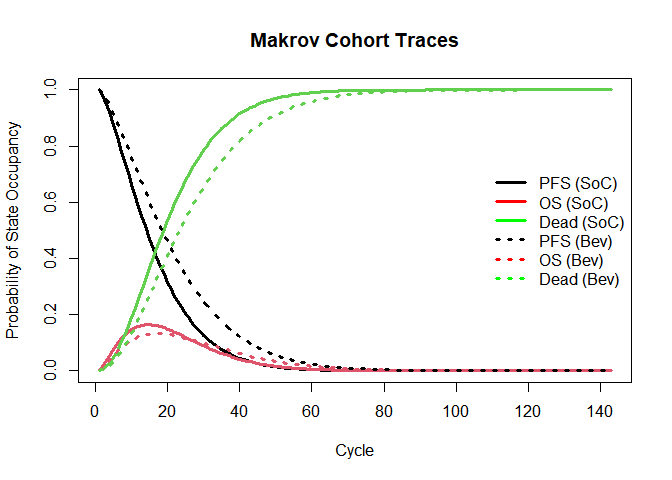
\includegraphics{Markov_3state_files/figure-latex/unnamed-chunk-25-1.pdf}

\hypertarget{two-way-sensitivity-analysis-twsa}{%
\subsection{08.4 Two-way sensitivity analysis
(TWSA)}\label{two-way-sensitivity-analysis-twsa}}

\begin{Shaded}
\begin{Highlighting}[]
\CommentTok{\# dataframe containing all parameters, their basecase values, and the min and }
\CommentTok{\# max values of the parameters of interest}
\NormalTok{df\_params\_twsa }\OtherTok{\textless{}{-}} \FunctionTok{data.frame}\NormalTok{(}\AttributeTok{pars =} \FunctionTok{c}\NormalTok{(}\StringTok{"c\_trtA"}\NormalTok{, }\StringTok{"c\_trtB"}\NormalTok{),}
                             \AttributeTok{min  =} \FunctionTok{c}\NormalTok{(}\DecValTok{300}\NormalTok{, }\DecValTok{500}\NormalTok{),  }\CommentTok{\# min parameter values}
                             \AttributeTok{max  =} \FunctionTok{c}\NormalTok{(}\DecValTok{1200}\NormalTok{, }\DecValTok{2000}\NormalTok{) }\CommentTok{\# max parameter values}
\NormalTok{)}

\NormalTok{twsa\_nmb }\OtherTok{\textless{}{-}} \FunctionTok{run\_twsa\_det}\NormalTok{(}\AttributeTok{params\_range    =}\NormalTok{ df\_params\_twsa,    }\CommentTok{\# dataframe with parameters for TWSA}
                         \AttributeTok{params\_basecase =}\NormalTok{ l\_params\_all,      }\CommentTok{\# list with all parameters}
                         \AttributeTok{nsamp           =} \DecValTok{40}\NormalTok{,                }\CommentTok{\# number of parameter values}
                         \AttributeTok{FUN             =}\NormalTok{ calculate\_ce\_out,  }\CommentTok{\# function to compute outputs}
                         \AttributeTok{outcomes        =} \StringTok{"NMB"}\NormalTok{,             }\CommentTok{\# output to do the TWSA on}
                         \AttributeTok{strategies      =}\NormalTok{ v\_names\_str,       }\CommentTok{\# names of the strategies}
                         \AttributeTok{n\_wtp           =} \DecValTok{5000}\NormalTok{)              }\CommentTok{\# extra argument to pass to FUN}
\end{Highlighting}
\end{Shaded}

\begin{verbatim}
##   |                                                                              |                                                                      |   0%  |                                                                              |                                                                      |   1%  |                                                                              |=                                                                     |   1%  |                                                                              |=                                                                     |   2%  |                                                                              |==                                                                    |   2%  |                                                                              |==                                                                    |   3%  |                                                                              |==                                                                    |   4%  |                                                                              |===                                                                   |   4%  |                                                                              |===                                                                   |   5%  |                                                                              |====                                                                  |   5%  |                                                                              |====                                                                  |   6%  |                                                                              |=====                                                                 |   6%  |                                                                              |=====                                                                 |   7%  |                                                                              |=====                                                                 |   8%  |                                                                              |======                                                                |   8%  |                                                                              |======                                                                |   9%  |                                                                              |=======                                                               |   9%  |                                                                              |=======                                                               |  10%  |                                                                              |=======                                                               |  11%  |                                                                              |========                                                              |  11%  |                                                                              |========                                                              |  12%  |                                                                              |=========                                                             |  12%  |                                                                              |=========                                                             |  13%  |                                                                              |=========                                                             |  14%  |                                                                              |==========                                                            |  14%  |                                                                              |==========                                                            |  15%  |                                                                              |===========                                                           |  15%  |                                                                              |===========                                                           |  16%  |                                                                              |============                                                          |  16%  |                                                                              |============                                                          |  17%  |                                                                              |============                                                          |  18%  |                                                                              |=============                                                         |  18%  |                                                                              |=============                                                         |  19%  |                                                                              |==============                                                        |  19%  |                                                                              |==============                                                        |  20%  |                                                                              |==============                                                        |  21%  |                                                                              |===============                                                       |  21%  |                                                                              |===============                                                       |  22%  |                                                                              |================                                                      |  22%  |                                                                              |================                                                      |  23%  |                                                                              |================                                                      |  24%  |                                                                              |=================                                                     |  24%  |                                                                              |=================                                                     |  25%  |                                                                              |==================                                                    |  25%  |                                                                              |==================                                                    |  26%  |                                                                              |===================                                                   |  26%  |                                                                              |===================                                                   |  27%  |                                                                              |===================                                                   |  28%  |                                                                              |====================                                                  |  28%  |                                                                              |====================                                                  |  29%  |                                                                              |=====================                                                 |  29%  |                                                                              |=====================                                                 |  30%  |                                                                              |=====================                                                 |  31%  |                                                                              |======================                                                |  31%  |                                                                              |======================                                                |  32%  |                                                                              |=======================                                               |  32%  |                                                                              |=======================                                               |  33%  |                                                                              |=======================                                               |  34%  |                                                                              |========================                                              |  34%  |                                                                              |========================                                              |  35%  |                                                                              |=========================                                             |  35%  |                                                                              |=========================                                             |  36%  |                                                                              |==========================                                            |  36%  |                                                                              |==========================                                            |  37%  |                                                                              |==========================                                            |  38%  |                                                                              |===========================                                           |  38%  |                                                                              |===========================                                           |  39%  |                                                                              |============================                                          |  39%  |                                                                              |============================                                          |  40%  |                                                                              |============================                                          |  41%  |                                                                              |=============================                                         |  41%  |                                                                              |=============================                                         |  42%  |                                                                              |==============================                                        |  42%  |                                                                              |==============================                                        |  43%  |                                                                              |==============================                                        |  44%  |                                                                              |===============================                                       |  44%  |                                                                              |===============================                                       |  45%  |                                                                              |================================                                      |  45%  |                                                                              |================================                                      |  46%  |                                                                              |=================================                                     |  46%  |                                                                              |=================================                                     |  47%  |                                                                              |=================================                                     |  48%  |                                                                              |==================================                                    |  48%  |                                                                              |==================================                                    |  49%  |                                                                              |===================================                                   |  49%  |                                                                              |===================================                                   |  50%  |                                                                              |===================================                                   |  51%  |                                                                              |====================================                                  |  51%  |                                                                              |====================================                                  |  52%  |                                                                              |=====================================                                 |  52%  |                                                                              |=====================================                                 |  53%  |                                                                              |=====================================                                 |  54%  |                                                                              |======================================                                |  54%  |                                                                              |======================================                                |  55%  |                                                                              |=======================================                               |  55%  |                                                                              |=======================================                               |  56%  |                                                                              |========================================                              |  56%  |                                                                              |========================================                              |  57%  |                                                                              |========================================                              |  58%  |                                                                              |=========================================                             |  58%  |                                                                              |=========================================                             |  59%  |                                                                              |==========================================                            |  59%  |                                                                              |==========================================                            |  60%  |                                                                              |==========================================                            |  61%  |                                                                              |===========================================                           |  61%  |                                                                              |===========================================                           |  62%  |                                                                              |============================================                          |  62%  |                                                                              |============================================                          |  63%  |                                                                              |============================================                          |  64%  |                                                                              |=============================================                         |  64%  |                                                                              |=============================================                         |  65%  |                                                                              |==============================================                        |  65%  |                                                                              |==============================================                        |  66%  |                                                                              |===============================================                       |  66%  |                                                                              |===============================================                       |  67%  |                                                                              |===============================================                       |  68%  |                                                                              |================================================                      |  68%  |                                                                              |================================================                      |  69%  |                                                                              |=================================================                     |  69%  |                                                                              |=================================================                     |  70%  |                                                                              |=================================================                     |  71%  |                                                                              |==================================================                    |  71%  |                                                                              |==================================================                    |  72%  |                                                                              |===================================================                   |  72%  |                                                                              |===================================================                   |  73%  |                                                                              |===================================================                   |  74%  |                                                                              |====================================================                  |  74%  |                                                                              |====================================================                  |  75%  |                                                                              |=====================================================                 |  75%  |                                                                              |=====================================================                 |  76%  |                                                                              |======================================================                |  76%  |                                                                              |======================================================                |  77%  |                                                                              |======================================================                |  78%  |                                                                              |=======================================================               |  78%  |                                                                              |=======================================================               |  79%  |                                                                              |========================================================              |  79%  |                                                                              |========================================================              |  80%  |                                                                              |========================================================              |  81%  |                                                                              |=========================================================             |  81%  |                                                                              |=========================================================             |  82%  |                                                                              |==========================================================            |  82%  |                                                                              |==========================================================            |  83%  |                                                                              |==========================================================            |  84%  |                                                                              |===========================================================           |  84%  |                                                                              |===========================================================           |  85%  |                                                                              |============================================================          |  85%  |                                                                              |============================================================          |  86%  |                                                                              |=============================================================         |  86%  |                                                                              |=============================================================         |  87%  |                                                                              |=============================================================         |  88%  |                                                                              |==============================================================        |  88%  |                                                                              |==============================================================        |  89%  |                                                                              |===============================================================       |  89%  |                                                                              |===============================================================       |  90%  |                                                                              |===============================================================       |  91%  |                                                                              |================================================================      |  91%  |                                                                              |================================================================      |  92%  |                                                                              |=================================================================     |  92%  |                                                                              |=================================================================     |  93%  |                                                                              |=================================================================     |  94%  |                                                                              |==================================================================    |  94%  |                                                                              |==================================================================    |  95%  |                                                                              |===================================================================   |  95%  |                                                                              |===================================================================   |  96%  |                                                                              |====================================================================  |  96%  |                                                                              |====================================================================  |  97%  |                                                                              |====================================================================  |  98%  |                                                                              |===================================================================== |  98%  |                                                                              |===================================================================== |  99%  |                                                                              |======================================================================|  99%  |                                                                              |======================================================================| 100%
\end{verbatim}

\hypertarget{plot-twsa}{%
\subsection{08.4.1 Plot TWSA}\label{plot-twsa}}

\begin{Shaded}
\begin{Highlighting}[]
\FunctionTok{plot}\NormalTok{(twsa\_nmb)}
\end{Highlighting}
\end{Shaded}

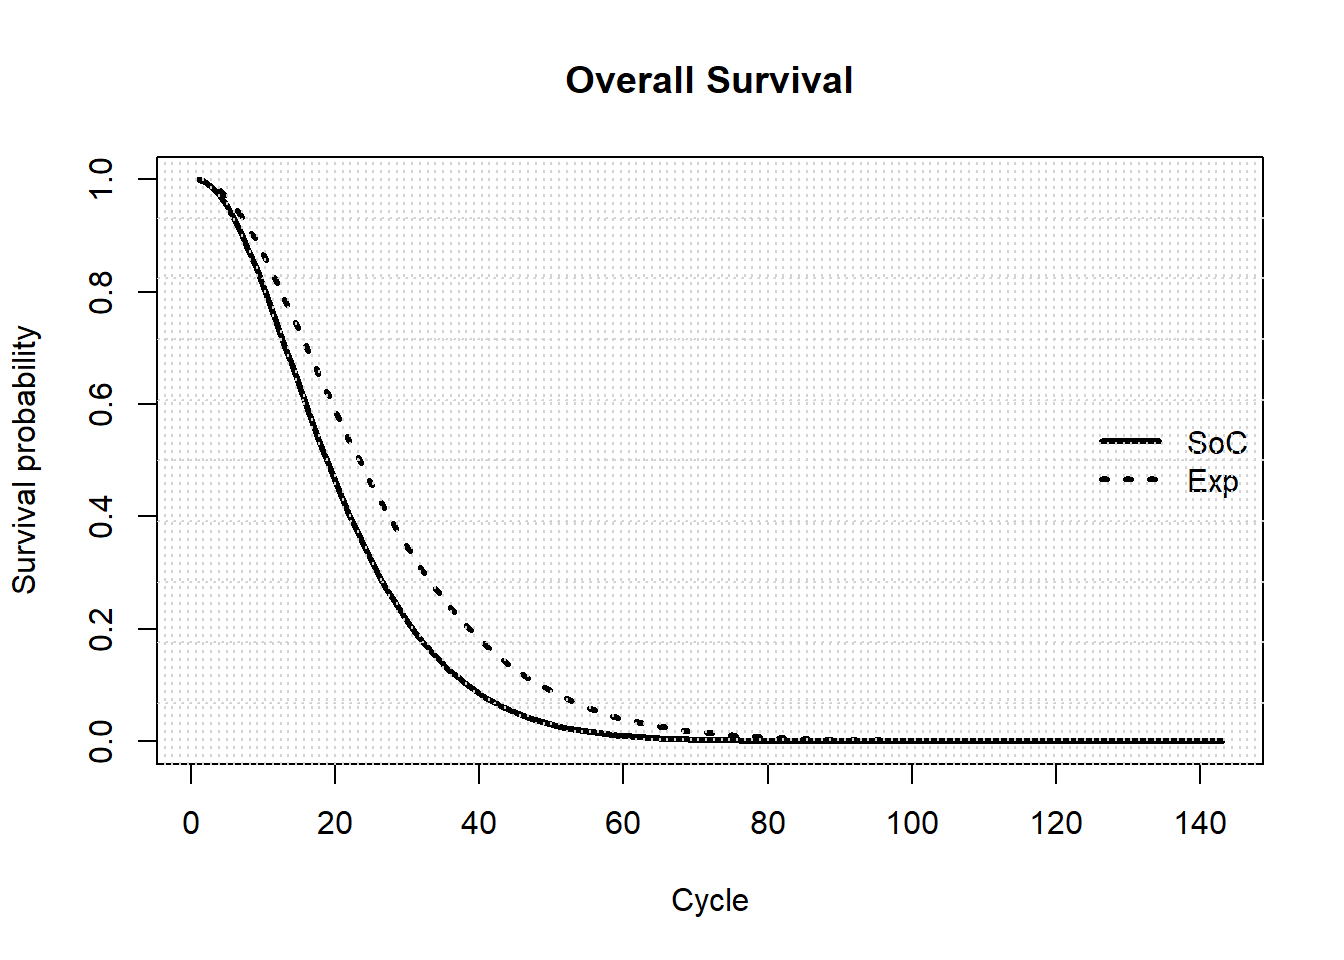
\includegraphics{Markov_3state_files/figure-latex/unnamed-chunk-27-1.pdf}

\hypertarget{probabilistic-sensitivity-analysis-psa}{%
\section{09 Probabilistic Sensitivity Analysis
(PSA)}\label{probabilistic-sensitivity-analysis-psa}}

\begin{Shaded}
\begin{Highlighting}[]
\CommentTok{\# Function to generate PSA input dataset}
\NormalTok{gen\_psa }\OtherTok{\textless{}{-}} \ControlFlowTok{function}\NormalTok{(}\AttributeTok{n\_sim =} \DecValTok{1000}\NormalTok{, }\AttributeTok{seed =} \DecValTok{071818}\NormalTok{)\{}
  \FunctionTok{set.seed}\NormalTok{(seed) }\CommentTok{\# set a seed to be able to reproduce the same results}
\NormalTok{  df\_psa }\OtherTok{\textless{}{-}} \FunctionTok{data.frame}\NormalTok{(}
    \CommentTok{\# Transition probabilities (per cycle), conditional on surviving}
    \CommentTok{\# probability to become PFS when OS}
    \CommentTok{\# probability of dying when OS}
    \AttributeTok{p\_HD       =} \FunctionTok{rbeta}\NormalTok{(n\_sim, }\AttributeTok{shape1 =} \DecValTok{4}\NormalTok{,  }\AttributeTok{shape2 =} \DecValTok{391}\NormalTok{),}
    \AttributeTok{p\_HS\_SoC   =} \FunctionTok{rbeta}\NormalTok{(n\_sim, }\AttributeTok{shape1 =} \DecValTok{24}\NormalTok{, }\AttributeTok{shape2 =} \DecValTok{450}\NormalTok{),  }\CommentTok{\# under standard of care}
    \AttributeTok{p\_HS\_trtA  =} \FunctionTok{rbeta}\NormalTok{(n\_sim, }\AttributeTok{shape1 =} \DecValTok{15}\NormalTok{, }\AttributeTok{shape2 =} \DecValTok{368}\NormalTok{),  }\CommentTok{\# under treatment A}
    \AttributeTok{p\_HS\_trtB  =} \FunctionTok{rbeta}\NormalTok{(n\_sim, }\AttributeTok{shape1 =} \DecValTok{16}\NormalTok{, }\AttributeTok{shape2 =} \DecValTok{767}\NormalTok{),  }\CommentTok{\# under treatment B}
    
    \CommentTok{\# probability of dying when PFS}
    \AttributeTok{p\_SD       =} \FunctionTok{rbeta}\NormalTok{(n\_sim, }\AttributeTok{shape1 =} \FloatTok{22.4}\NormalTok{, }\AttributeTok{shape2 =} \FloatTok{201.6}\NormalTok{), }
    
    \CommentTok{\# Cost vectors with length n\_sim}
    \CommentTok{\# cost of remaining one cycle in state H}
    \AttributeTok{c\_H        =} \FunctionTok{rgamma}\NormalTok{(n\_sim, }\AttributeTok{shape =} \DecValTok{16}\NormalTok{, }\AttributeTok{scale =} \DecValTok{25}\NormalTok{), }
    \CommentTok{\# cost of remaining one cycle in state S1}
    \AttributeTok{c\_S        =} \FunctionTok{rgamma}\NormalTok{(n\_sim, }\AttributeTok{shape =} \DecValTok{100}\NormalTok{, }\AttributeTok{scale =} \DecValTok{10}\NormalTok{), }
    \CommentTok{\# cost of being in the death state}
    \AttributeTok{c\_D        =} \DecValTok{0}\NormalTok{, }
    \CommentTok{\# cost of treatment (per cycle)}
    \AttributeTok{c\_trtA    =} \FunctionTok{rgamma}\NormalTok{(n\_sim, }\AttributeTok{shape =} \DecValTok{64}\NormalTok{, }\AttributeTok{scale =} \FloatTok{12.5}\NormalTok{),}
    \CommentTok{\# cost of treatment (per cycle)}
    \AttributeTok{c\_trtB    =} \FunctionTok{rgamma}\NormalTok{(n\_sim, }\AttributeTok{shape =} \DecValTok{225}\NormalTok{, }\AttributeTok{scale =} \FloatTok{6.67}\NormalTok{),}
    
    \CommentTok{\# Utility vectors with length n\_sim }
    \CommentTok{\# utility when OS}
    \AttributeTok{u\_H        =} \FunctionTok{rbeta}\NormalTok{(n\_sim, }\AttributeTok{shape1 =}  \FloatTok{1.5}\NormalTok{, }\AttributeTok{shape2 =} \FloatTok{0.0015}\NormalTok{), }
    \CommentTok{\# utility when PFS}
    \AttributeTok{u\_S        =} \FunctionTok{rbeta}\NormalTok{(n\_sim, }\AttributeTok{shape1 =} \FloatTok{49.5}\NormalTok{, }\AttributeTok{shape2 =} \FloatTok{49.5}\NormalTok{), }
    \CommentTok{\# utility when dead}
    \AttributeTok{u\_D        =} \DecValTok{0}                                              
\NormalTok{  )}
  \FunctionTok{return}\NormalTok{(df\_psa)}
\NormalTok{\}}


\CommentTok{\# Try it}
\FunctionTok{gen\_psa}\NormalTok{(}\DecValTok{10}\NormalTok{) }
\end{Highlighting}
\end{Shaded}

\begin{verbatim}
##           p_HD   p_HS_SoC  p_HS_trtA  p_HS_trtB       p_SD      c_H       c_S
## 1  0.010409832 0.03864534 0.05106946 0.01880191 0.08716784 473.5520 1080.4473
## 2  0.005787008 0.05803256 0.05374466 0.03663437 0.08683307 390.7068  984.6521
## 3  0.011628880 0.04043569 0.02971281 0.02665266 0.12125280 393.7788  820.5960
## 4  0.004206986 0.07272604 0.05047031 0.01737607 0.07939792 388.4159 1138.0161
## 5  0.008707210 0.04204598 0.03827582 0.02249263 0.09201305 348.6654  858.9336
## 6  0.008811813 0.06282706 0.02893692 0.02755339 0.08836480 383.0443 1066.2746
## 7  0.006723925 0.04844997 0.02850594 0.01771985 0.09186392 337.9317 1056.6110
## 8  0.011441452 0.06899590 0.04088357 0.01055079 0.11862418 375.8565 1061.5311
## 9  0.002780751 0.05355168 0.03261544 0.03693418 0.09201745 443.4329 1193.5129
## 10 0.008215617 0.03351956 0.03799814 0.02147359 0.10253465 265.5241  800.1153
##    c_D    c_trtA   c_trtB u_H       u_S u_D
## 1    0  757.1225 1530.270   1 0.4289183   0
## 2    0  787.5281 1530.355   1 0.4406711   0
## 3    0  692.5136 1537.820   1 0.5685309   0
## 4    0  725.4467 1561.473   1 0.5259122   0
## 5    0  618.2429 1540.150   1 0.6263893   0
## 6    0 1021.4048 1519.897   1 0.5488176   0
## 7    0  757.4433 1407.022   1 0.4941487   0
## 8    0  768.0045 1600.675   1 0.4764772   0
## 9    0  966.1955 1540.285   1 0.6021962   0
## 10   0  863.7855 1632.233   1 0.4743638   0
\end{verbatim}

\begin{Shaded}
\begin{Highlighting}[]
\CommentTok{\# Number of simulations}
\NormalTok{n\_sim }\OtherTok{\textless{}{-}} \DecValTok{1000}

\CommentTok{\# Generate PSA input dataset}
\NormalTok{df\_psa\_input }\OtherTok{\textless{}{-}} \FunctionTok{gen\_psa}\NormalTok{(}\AttributeTok{n\_sim =}\NormalTok{ n\_sim)}
\CommentTok{\# First six observations}
\FunctionTok{head}\NormalTok{(df\_psa\_input)}
\end{Highlighting}
\end{Shaded}

\begin{verbatim}
##          p_HD   p_HS_SoC  p_HS_trtA  p_HS_trtB       p_SD      c_H       c_S
## 1 0.010409832 0.05171914 0.03970387 0.02225447 0.12518814 212.2816 1137.1008
## 2 0.005787008 0.06436450 0.03248900 0.01515043 0.09693103 369.9141  958.1121
## 3 0.011628880 0.03903574 0.03946831 0.02429807 0.09261952 297.5068 1209.0566
## 4 0.004206986 0.05192643 0.03004580 0.02021414 0.07760384 514.2313  977.5293
## 5 0.008707210 0.04663933 0.02881959 0.02190302 0.11585757 382.7674 1023.0726
## 6 0.008811813 0.03871080 0.03325803 0.01292004 0.12174825 452.0530 1132.4417
##   c_D   c_trtA   c_trtB u_H       u_S u_D
## 1   0 755.4064 1516.060   1 0.5448863   0
## 2   0 789.3537 1371.786   1 0.5986094   0
## 3   0 994.7402 1523.188   1 0.5092672   0
## 4   0 739.4736 1561.273   1 0.4486940   0
## 5   0 893.4923 1352.092   1 0.5286213   0
## 6   0 881.5849 1660.185   1 0.6005060   0
\end{verbatim}

\begin{Shaded}
\begin{Highlighting}[]
\CommentTok{\# Save the dataframe}
\CommentTok{\# save dataframe}
\CommentTok{\#save(df\_psa\_input, file = "df\_psa\_input.rda")}


\CommentTok{\# Histogram of parameters}
\FunctionTok{ggplot}\NormalTok{(}\FunctionTok{melt}\NormalTok{(df\_psa\_input, }\AttributeTok{variable.name =} \StringTok{"Parameter"}\NormalTok{), }\FunctionTok{aes}\NormalTok{(}\AttributeTok{x =}\NormalTok{ value)) }\SpecialCharTok{+}
  \FunctionTok{facet\_wrap}\NormalTok{(}\SpecialCharTok{\textasciitilde{}}\NormalTok{Parameter, }\AttributeTok{scales =} \StringTok{"free"}\NormalTok{) }\SpecialCharTok{+}
  \FunctionTok{geom\_histogram}\NormalTok{(}\FunctionTok{aes}\NormalTok{(}\AttributeTok{y =}\NormalTok{ ..density..)) }\SpecialCharTok{+}
  \FunctionTok{theme\_bw}\NormalTok{(}\AttributeTok{base\_size =} \DecValTok{16}\NormalTok{) }\SpecialCharTok{+} 
  \FunctionTok{theme}\NormalTok{(}\AttributeTok{axis.text =} \FunctionTok{element\_text}\NormalTok{(}\AttributeTok{size=}\DecValTok{8}\NormalTok{))}
\end{Highlighting}
\end{Shaded}

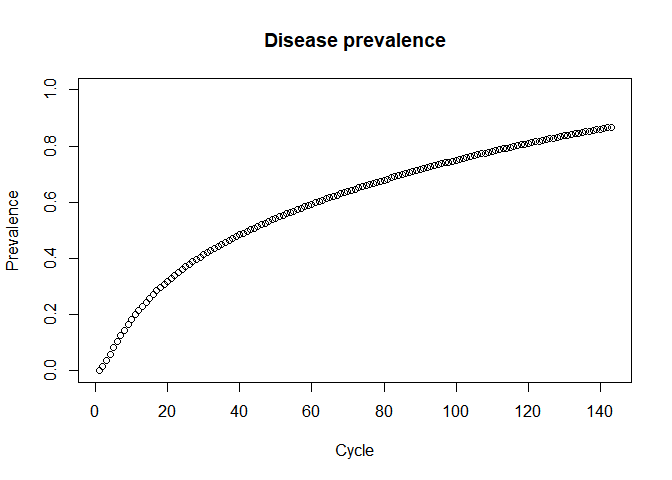
\includegraphics{Markov_3state_files/figure-latex/unnamed-chunk-28-1.pdf}

\begin{Shaded}
\begin{Highlighting}[]
\CommentTok{\# Initialize dataframes with PSA output }
\CommentTok{\# Dataframe of costs}
\NormalTok{df\_c }\OtherTok{\textless{}{-}} \FunctionTok{as.data.frame}\NormalTok{(}\FunctionTok{matrix}\NormalTok{(}\DecValTok{0}\NormalTok{, }
                             \AttributeTok{nrow =}\NormalTok{ n\_sim,}
                             \AttributeTok{ncol =}\NormalTok{ n\_str))}
\FunctionTok{colnames}\NormalTok{(df\_c) }\OtherTok{\textless{}{-}}\NormalTok{ v\_names\_str}
\CommentTok{\# Dataframe of effectiveness}
\NormalTok{df\_e }\OtherTok{\textless{}{-}} \FunctionTok{as.data.frame}\NormalTok{(}\FunctionTok{matrix}\NormalTok{(}\DecValTok{0}\NormalTok{, }
                             \AttributeTok{nrow =}\NormalTok{ n\_sim,}
                             \AttributeTok{ncol =}\NormalTok{ n\_str))}
\FunctionTok{colnames}\NormalTok{(df\_e) }\OtherTok{\textless{}{-}}\NormalTok{ v\_names\_str}
\end{Highlighting}
\end{Shaded}

I need to fix the ``\# Histogram of parameters'' section above, the
below gives advice on doing this:

\url{https://stackoverflow.com/questions/68416435/rcpp-package-doesnt-include-rcpp-precious-remove}

\url{https://www.mail-archive.com/rcpp-devel@lists.r-forge.r-project.org/msg10226.html}

\url{https://statisticsglobe.com/warning-cannot-remove-prior-installation-in-r}

The above approach worked, I manually deleted the package, installed
darthtools from github, chose option 4, i.e.~replace rccp and then I was
done.

\hypertarget{conduct-probabilistic-sensitivity-analysis}{%
\subsection{09.1 Conduct probabilistic sensitivity
analysis}\label{conduct-probabilistic-sensitivity-analysis}}

\begin{Shaded}
\begin{Highlighting}[]
\CommentTok{\# Run Markov model on each parameter set of PSA input dataset}
\ControlFlowTok{for}\NormalTok{(i }\ControlFlowTok{in} \DecValTok{1}\SpecialCharTok{:}\NormalTok{n\_sim)\{}
\NormalTok{  l\_out\_temp }\OtherTok{\textless{}{-}} \FunctionTok{calculate\_ce\_out}\NormalTok{(df\_psa\_input[i, ])}
\NormalTok{  df\_c[i, ] }\OtherTok{\textless{}{-}}\NormalTok{ l\_out\_temp}\SpecialCharTok{$}\NormalTok{Cost}
\NormalTok{  df\_e[i, ] }\OtherTok{\textless{}{-}}\NormalTok{ l\_out\_temp}\SpecialCharTok{$}\NormalTok{Effect}
  \CommentTok{\# Display simulation progress}
  \ControlFlowTok{if}\NormalTok{(i}\SpecialCharTok{/}\NormalTok{(n\_sim}\SpecialCharTok{/}\DecValTok{10}\NormalTok{) }\SpecialCharTok{==} \FunctionTok{round}\NormalTok{(i}\SpecialCharTok{/}\NormalTok{(n\_sim}\SpecialCharTok{/}\DecValTok{10}\NormalTok{), }\DecValTok{0}\NormalTok{)) \{ }\CommentTok{\# display progress every 10\%}
    \FunctionTok{cat}\NormalTok{(}\StringTok{\textquotesingle{}}\SpecialCharTok{\textbackslash{}r}\StringTok{\textquotesingle{}}\NormalTok{, }\FunctionTok{paste}\NormalTok{(i}\SpecialCharTok{/}\NormalTok{n\_sim }\SpecialCharTok{*} \DecValTok{100}\NormalTok{, }\StringTok{"\% done"}\NormalTok{, }\AttributeTok{sep =} \StringTok{" "}\NormalTok{))}
\NormalTok{  \}}
\NormalTok{\}}
\end{Highlighting}
\end{Shaded}

\begin{verbatim}
##  10 % done 20 % done 30 % done 40 % done 50 % done 60 % done 70 % done 80 % done 90 % done 100 % done
\end{verbatim}

\hypertarget{create-psa-object-for-dampack}{%
\subsection{09.2 Create PSA object for
dampack}\label{create-psa-object-for-dampack}}

\begin{Shaded}
\begin{Highlighting}[]
\NormalTok{l\_psa }\OtherTok{\textless{}{-}} \FunctionTok{make\_psa\_obj}\NormalTok{(}\AttributeTok{cost          =}\NormalTok{ df\_c, }
                      \AttributeTok{effectiveness =}\NormalTok{ df\_e, }
                      \AttributeTok{parameters    =}\NormalTok{ df\_psa\_input, }
                      \AttributeTok{strategies    =}\NormalTok{ v\_names\_str)}
\end{Highlighting}
\end{Shaded}

\hypertarget{save-psa-objects}{%
\subsection{09.2.1 Save PSA objects}\label{save-psa-objects}}

\begin{Shaded}
\begin{Highlighting}[]
\FunctionTok{save}\NormalTok{(df\_psa\_input, df\_c, df\_e, v\_names\_str, n\_str, l\_psa,}
     \AttributeTok{file =} \StringTok{"markov\_3state\_PSA\_dataset.RData"}\NormalTok{)}
\end{Highlighting}
\end{Shaded}

Vector with willingness-to-pay (WTP) thresholds.

\begin{Shaded}
\begin{Highlighting}[]
\NormalTok{v\_wtp }\OtherTok{\textless{}{-}} \FunctionTok{seq}\NormalTok{(}\DecValTok{0}\NormalTok{, }\DecValTok{30000}\NormalTok{, }\AttributeTok{by =} \DecValTok{1000}\NormalTok{)}
\end{Highlighting}
\end{Shaded}

\hypertarget{cost-effectiveness-scatter-plot}{%
\subsection{09.3.1 Cost-Effectiveness Scatter
plot}\label{cost-effectiveness-scatter-plot}}

\begin{Shaded}
\begin{Highlighting}[]
\FunctionTok{plot}\NormalTok{(l\_psa, }\AttributeTok{xlim =} \FunctionTok{c}\NormalTok{(}\FloatTok{9.5}\NormalTok{, }\FloatTok{22.5}\NormalTok{))}
\end{Highlighting}
\end{Shaded}

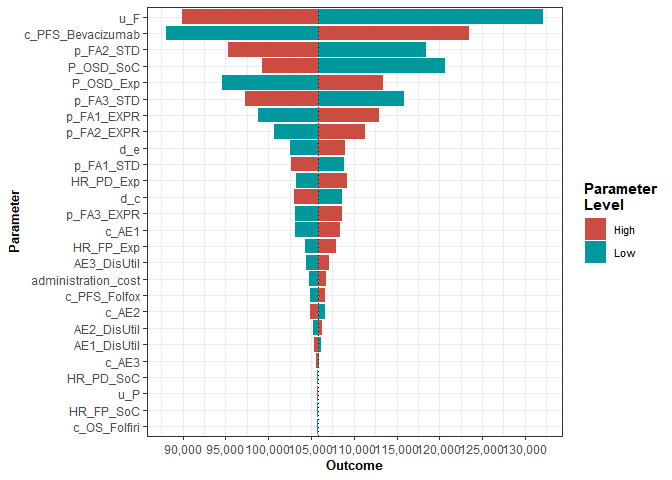
\includegraphics{Markov_3state_files/figure-latex/unnamed-chunk-33-1.pdf}

\hypertarget{conduct-cea-with-probabilistic-output}{%
\subsection{09.4 Conduct CEA with probabilistic
output}\label{conduct-cea-with-probabilistic-output}}

\begin{Shaded}
\begin{Highlighting}[]
\CommentTok{\# Compute expected costs and effects for each strategy from the PSA}
\NormalTok{df\_out\_ce\_psa }\OtherTok{\textless{}{-}} \FunctionTok{summary}\NormalTok{(l\_psa)}

\CommentTok{\# Calculate incremental cost{-}effectiveness ratios (ICERs)}
\NormalTok{df\_cea\_psa }\OtherTok{\textless{}{-}} \FunctionTok{calculate\_icers}\NormalTok{(}\AttributeTok{cost       =}\NormalTok{ df\_out\_ce\_psa}\SpecialCharTok{$}\NormalTok{meanCost, }
                              \AttributeTok{effect     =}\NormalTok{ df\_out\_ce\_psa}\SpecialCharTok{$}\NormalTok{meanEffect,}
                              \AttributeTok{strategies =}\NormalTok{ df\_out\_ce\_psa}\SpecialCharTok{$}\NormalTok{Strategy)}
\NormalTok{df\_cea\_psa}
\end{Highlighting}
\end{Shaded}

\begin{verbatim}
##           Strategy      Cost  Effect Inc_Cost Inc_Effect     ICER Status
## 1 Standard.of.Care  9000.388 13.6749       NA         NA       NA     ND
## 2        HDX.Assay 34432.974 18.0447 25432.59   4.369801 5820.079     ND
## 3        EPI.Assay 19502.504 14.9531       NA         NA       NA     ED
\end{verbatim}

\begin{Shaded}
\begin{Highlighting}[]
\CommentTok{\# Save CEA table with ICERs}
\CommentTok{\# As .RData}
\FunctionTok{save}\NormalTok{(df\_cea\_psa, }
     \AttributeTok{file =} \StringTok{"markov\_3state\_probabilistic\_CEA\_results.RData"}\NormalTok{)}
\CommentTok{\# As .csv}
\FunctionTok{write.csv}\NormalTok{(df\_cea\_psa, }
          \AttributeTok{file =} \StringTok{"markov\_3state\_probabilistic\_CEA\_results.csv"}\NormalTok{)}
\end{Highlighting}
\end{Shaded}

\hypertarget{plot-cost-effectiveness-frontier}{%
\subsection{09.4.1 Plot cost-effectiveness
frontier}\label{plot-cost-effectiveness-frontier}}

\begin{Shaded}
\begin{Highlighting}[]
\FunctionTok{plot}\NormalTok{(df\_cea\_psa)}
\end{Highlighting}
\end{Shaded}

\includegraphics{Markov_3state_files/figure-latex/unnamed-chunk-35-1.pdf}

\hypertarget{cost-effectiveness-acceptability-curves-ceacs-and-frontier-ceaf}{%
\subsection{09.4.2 Cost-effectiveness acceptability curves (CEACs) and
frontier
(CEAF)}\label{cost-effectiveness-acceptability-curves-ceacs-and-frontier-ceaf}}

\begin{Shaded}
\begin{Highlighting}[]
\NormalTok{ceac\_obj }\OtherTok{\textless{}{-}} \FunctionTok{ceac}\NormalTok{(}\AttributeTok{wtp =}\NormalTok{ v\_wtp, }\AttributeTok{psa =}\NormalTok{ l\_psa)}
\CommentTok{\# Regions of highest probability of cost{-}effectiveness for each strategy}
\FunctionTok{summary}\NormalTok{(ceac\_obj)}
\end{Highlighting}
\end{Shaded}

\begin{verbatim}
##   range_min range_max   cost_eff_strat
## 1         0      6000 Standard.of.Care
## 2      6000     30000        HDX.Assay
\end{verbatim}

\begin{Shaded}
\begin{Highlighting}[]
\CommentTok{\# CEAC \& CEAF plot}
\FunctionTok{plot}\NormalTok{(ceac\_obj)}
\end{Highlighting}
\end{Shaded}

\includegraphics{Markov_3state_files/figure-latex/unnamed-chunk-36-1.pdf}

\hypertarget{expected-loss-curves-elcs}{%
\subsection{09.4.3 Expected Loss Curves
(ELCs)}\label{expected-loss-curves-elcs}}

The expected loss is the the quantification of the foregone benefits
when choosing a suboptimal strategy given current evidence.

\begin{Shaded}
\begin{Highlighting}[]
\NormalTok{elc\_obj }\OtherTok{\textless{}{-}} \FunctionTok{calc\_exp\_loss}\NormalTok{(}\AttributeTok{wtp =}\NormalTok{ v\_wtp, }\AttributeTok{psa =}\NormalTok{ l\_psa)}
\NormalTok{elc\_obj}
\end{Highlighting}
\end{Shaded}

\begin{verbatim}
##      WTP         Strategy Expected_Loss On_Frontier
## 1      0 Standard.of.Care       0.00000        TRUE
## 2      0        EPI.Assay   10502.11619       FALSE
## 3      0        HDX.Assay   25432.58610       FALSE
## 4   1000 Standard.of.Care       0.00000        TRUE
## 5   1000        EPI.Assay    9223.92409       FALSE
## 6   1000        HDX.Assay   21062.78542       FALSE
## 7   2000 Standard.of.Care       0.00000        TRUE
## 8   2000        EPI.Assay    7945.73200       FALSE
## 9   2000        HDX.Assay   16692.98473       FALSE
## 10  3000 Standard.of.Care      79.25557        TRUE
## 11  3000        EPI.Assay    6746.79547       FALSE
## 12  3000        HDX.Assay   12402.43961       FALSE
## 13  4000 Standard.of.Care     562.36838        TRUE
## 14  4000        EPI.Assay    5951.71617       FALSE
## 15  4000        HDX.Assay    8515.75173       FALSE
## 16  5000 Standard.of.Care    2025.57054        TRUE
## 17  5000        EPI.Assay    6136.72624       FALSE
## 18  5000        HDX.Assay    5609.15321       FALSE
## 19  6000 Standard.of.Care    4564.24629       FALSE
## 20  6000        EPI.Assay    7397.20989       FALSE
## 21  6000        HDX.Assay    3778.02827        TRUE
## 22  7000 Standard.of.Care    7883.62541       FALSE
## 23  7000        EPI.Assay    9438.39691       FALSE
## 24  7000        HDX.Assay    2727.60670        TRUE
## 25  8000 Standard.of.Care   11627.98059       FALSE
## 26  8000        EPI.Assay   11904.55999       FALSE
## 27  8000        HDX.Assay    2102.16119        TRUE
## 28  9000 Standard.of.Care   15623.39251       FALSE
## 29  9000        EPI.Assay   14621.77981       FALSE
## 30  9000        HDX.Assay    1727.77242        TRUE
## 31 10000 Standard.of.Care   19764.99430       FALSE
## 32 10000        EPI.Assay   17485.18950       FALSE
## 33 10000        HDX.Assay    1499.57352        TRUE
## 34 11000 Standard.of.Care   23981.66842       FALSE
## 35 11000        EPI.Assay   20423.67153       FALSE
## 36 11000        HDX.Assay    1346.44696        TRUE
## 37 12000 Standard.of.Care   28242.26849       FALSE
## 38 12000        EPI.Assay   23406.07949       FALSE
## 39 12000        HDX.Assay    1237.24633        TRUE
## 40 13000 Standard.of.Care   32529.07107       FALSE
## 41 13000        EPI.Assay   26414.68998       FALSE
## 42 13000        HDX.Assay    1154.24823        TRUE
## 43 14000 Standard.of.Care   36836.42889       FALSE
## 44 14000        EPI.Assay   29443.85569       FALSE
## 45 14000        HDX.Assay    1091.80536        TRUE
## 46 15000 Standard.of.Care   41154.74763       FALSE
## 47 15000        EPI.Assay   32483.98234       FALSE
## 48 15000        HDX.Assay    1040.32341        TRUE
## 49 16000 Standard.of.Care   45482.87736       FALSE
## 50 16000        EPI.Assay   35533.91997       FALSE
## 51 16000        HDX.Assay     998.65245        TRUE
## 52 17000 Standard.of.Care   49821.95879       FALSE
## 53 17000        EPI.Assay   38594.80930       FALSE
## 54 17000        HDX.Assay     967.93319        TRUE
## 55 18000 Standard.of.Care   54168.47343       FALSE
## 56 18000        EPI.Assay   41663.13184       FALSE
## 57 18000        HDX.Assay     944.64715        TRUE
## 58 19000 Standard.of.Care   58517.73380       FALSE
## 59 19000        EPI.Assay   44734.20011       FALSE
## 60 19000        HDX.Assay     924.10683        TRUE
## 61 20000 Standard.of.Care   62871.54306       FALSE
## 62 20000        EPI.Assay   47809.81727       FALSE
## 63 20000        HDX.Assay     908.11540        TRUE
## 64 21000 Standard.of.Care   67230.89679       FALSE
## 65 21000        EPI.Assay   50890.97890       FALSE
## 66 21000        HDX.Assay     897.66844        TRUE
## 67 22000 Standard.of.Care   71596.69192       FALSE
## 68 22000        EPI.Assay   53978.58193       FALSE
## 69 22000        HDX.Assay     893.66289        TRUE
## 70 23000 Standard.of.Care   75965.74328       FALSE
## 71 23000        EPI.Assay   57069.44119       FALSE
## 72 23000        HDX.Assay     892.91356        TRUE
## 73 24000 Standard.of.Care   80336.91054       FALSE
## 74 24000        EPI.Assay   60162.41635       FALSE
## 75 24000        HDX.Assay     894.28013        TRUE
## 76 25000 Standard.of.Care   84709.17443       FALSE
## 77 25000        EPI.Assay   63256.48814       FALSE
## 78 25000        HDX.Assay     896.74333        TRUE
## 79 26000 Standard.of.Care   89082.19327       FALSE
## 80 26000        EPI.Assay   66351.31488       FALSE
## 81 26000        HDX.Assay     899.96148        TRUE
## 82 27000 Standard.of.Care   93456.95920       FALSE
## 83 27000        EPI.Assay   69447.88872       FALSE
## 84 27000        HDX.Assay     904.92673        TRUE
## 85 28000 Standard.of.Care   97834.11366       FALSE
## 86 28000        EPI.Assay   72546.85108       FALSE
## 87 28000        HDX.Assay     912.28050        TRUE
## 88 29000 Standard.of.Care  102212.03809       FALSE
## 89 29000        EPI.Assay   75646.58341       FALSE
## 90 29000        HDX.Assay     920.40424        TRUE
## 91 30000 Standard.of.Care  106591.23912       FALSE
## 92 30000        EPI.Assay   78747.59233       FALSE
## 93 30000        HDX.Assay     929.80458        TRUE
\end{verbatim}

\begin{Shaded}
\begin{Highlighting}[]
\CommentTok{\# ELC plot}
\FunctionTok{plot}\NormalTok{(elc\_obj, }\AttributeTok{log\_y =} \ConstantTok{FALSE}\NormalTok{)}
\end{Highlighting}
\end{Shaded}

\includegraphics{Markov_3state_files/figure-latex/unnamed-chunk-37-1.pdf}

\hypertarget{expected-value-of-perfect-information-evpi}{%
\subsection{09.4.4 Expected value of perfect information
(EVPI)}\label{expected-value-of-perfect-information-evpi}}

Value of information is discussed in the York course and below:

C:\Users\Jonathan\OneDrive - Royal College of Surgeons in
Ireland\COLOSSUS\Training Resources\CDC\_Exclusive\_Decision Modeling
for Public Health\_DARTH

\begin{Shaded}
\begin{Highlighting}[]
\NormalTok{evpi }\OtherTok{\textless{}{-}} \FunctionTok{calc\_evpi}\NormalTok{(}\AttributeTok{wtp =}\NormalTok{ v\_wtp, }\AttributeTok{psa =}\NormalTok{ l\_psa)}
\CommentTok{\# EVPI plot}
\FunctionTok{plot}\NormalTok{(evpi, }\AttributeTok{effect\_units =} \StringTok{"QALY"}\NormalTok{)}
\end{Highlighting}
\end{Shaded}

\includegraphics{Markov_3state_files/figure-latex/unnamed-chunk-38-1.pdf}

\hypertarget{references}{%
\subsection{References:}\label{references}}

Useful Darth publications to cite when using this code:

\begin{itemize}
\item
  Jalal H, Pechlivanoglou P, Krijkamp E, Alarid-Escudero F, Enns E,
  Hunink MG. An Overview of R in Health Decision Sciences. Med Decis
  Making. 2017; 37(3): 735-746.
  \url{https://journals.sagepub.com/doi/abs/10.1177/0272989X16686559}
\item
  Alarid-Escudero F, Krijkamp EM, Enns EA, Yang A, Hunink MGM
  Pechlivanoglou P, Jalal H. Cohort State-Transition Models in R: A
  Tutorial. arXiv:200107824v2. 2020:1-48.
  \url{http://arxiv.org/abs/2001.07824}
\item
  Krijkamp EM, Alarid-Escudero F, Enns EA, Jalal HJ, Hunink MGM,
  Pechlivanoglou P. Microsimulation modeling for health decision
  sciences using R: A tutorial. Med Decis Making. 2018;38(3):400--22.
  \url{https://journals.sagepub.com/doi/abs/10.1177/0272989X18754513}
\item
  Krijkamp EM, Alarid-Escudero F, Enns E, Pechlivanoglou P, Hunink MM,
  Jalal H. A Multidimensional Array Representation of State-Transition
  Model Dynamics. Med Decis Making. Online First
  \url{https://doi.org/10.1177/0272989X19893973}
\end{itemize}

\hypertarget{refs}{}
\begin{CSLReferences}{1}{0}
\leavevmode\hypertarget{ref-alarid-escudero2021}{}%
Alarid-Escudero, Fernando, Eline M. Krijkamp, Eva A. Enns, Alan Yang, M.
G. Myriam Hunink, Petros Pechlivanoglou, and Hawre Jalal. 2021. {``An
Introductory Tutorial on Cohort State-Transition Models in r Using a
Cost-Effectiveness Analysis Example.''} \emph{arXiv:2001.07824 {[}q-Bio,
Stat{]}}, August. \url{http://arxiv.org/abs/2001.07824}.

\leavevmode\hypertarget{ref-dekker2019}{}%
Dekker, Evelien, Pieter J. Tanis, Jasper L. A. Vleugels, Pashtoon M.
Kasi, and Michael B. Wallace. 2019. {``Colorectal Cancer.''} \emph{The
Lancet} 394 (10207): 1467--80.
\url{https://doi.org/10.1016/S0140-6736(19)32319-0}.

\leavevmode\hypertarget{ref-goldstein2014}{}%
Goldstein, Daniel A., Qiushi Chen, Turgay Ayer, David H. Howard, Joseph
Lipscomb, R. Donald Harvey, Bassel F. El-Rayes, and Christopher R.
Flowers. 2014. {``Cost Effectiveness Analysis of
Pharmacokinetically-Guided 5-Fluorouracil in FOLFOX Chemotherapy for
Metastatic Colorectal Cancer.''} \emph{Clinical Colorectal Cancer} 13
(4): 219--25. \url{https://doi.org/10.1016/j.clcc.2014.09.007}.

\leavevmode\hypertarget{ref-jalal2017}{}%
Jalal, Hawre, Petros Pechlivanoglou, Eline Krijkamp, Fernando
Alarid-Escudero, Eva Enns, and M. G. Myriam Hunink. 2017. {``An Overview
of R in Health Decision Sciences.''} \emph{Medical Decision Making} 37
(7): 735--46. \url{https://doi.org/10.1177/0272989X16686559}.

\leavevmode\hypertarget{ref-krijkamp2018}{}%
Krijkamp, Eline M., Fernando Alarid-Escudero, Eva A. Enns, Hawre J.
Jalal, M. G. Myriam Hunink, and Petros Pechlivanoglou. 2018.
{``Microsimulation Modeling for Health Decision Sciences Using R: A
Tutorial.''} \emph{Medical Decision Making} 38 (3): 400--422.
\url{https://doi.org/10.1177/0272989X18754513}.

\leavevmode\hypertarget{ref-krijkamp2020}{}%
Krijkamp, Eline M., Fernando Alarid-Escudero, Eva A. Enns, Petros
Pechlivanoglou, M.G. Myriam Hunink, Alan Yang, and Hawre J. Jalal. 2020.
{``A Multidimensional Array Representation of State-Transition Model
Dynamics.''} \emph{Medical Decision Making} 40 (2): 242--48.
\url{https://doi.org/10.1177/0272989X19893973}.

\leavevmode\hypertarget{ref-nwaokorie2021}{}%
Nwaokorie, Annabelle, and Dirk Fey. 2021. {``Personalised Medicine for
Colorectal Cancer Using Mechanism-Based Machine Learning Models.''}
\emph{International Journal of Molecular Sciences} 22 (18): 9970.
\url{https://doi.org/10.3390/ijms22189970}.

\leavevmode\hypertarget{ref-patelli2021}{}%
Patelli, G., F. Tosi, A. Amatu, G. Mauri, A. Curaba, D.A. Patanè, A.
Pani, F. Scaglione, S. Siena, and A. Sartore-Bianchi. 2021.
{``Strategies to Tackle RAS-Mutated Metastatic Colorectal Cancer.''}
\emph{ESMO Open} 6 (3): 100156.
\url{https://doi.org/10.1016/j.esmoop.2021.100156}.

\leavevmode\hypertarget{ref-ramsey2000}{}%
Ramsey, Scott D., M. Robyn Andersen, Ruth Etzioni, Carol Moinpour, Sue
Peacock, Arnold Potosky, and Nicole Urban. 2000. {``Quality of Life in
Survivors of Colorectal Carcinoma.''} \emph{Cancer} 88 (6): 1294--1303.
https://doi.org/\url{https://doi.org/10.1002/(SICI)1097-0142(20000315)88:6\%3C1294::AID-CNCR4\%3E3.0.CO;2-M}.

\leavevmode\hypertarget{ref-siegel2019}{}%
Siegel, Rebecca L., Kimberly D. Miller, and Ahmedin Jemal. 2019.
{``Cancer Statistics, 2019.''} \emph{CA: A Cancer Journal for
Clinicians} 69 (1): 734.

\leavevmode\hypertarget{ref-tiwari2018}{}%
Tiwari, Ankita, Shivani Saraf, Amit Verma, Pritish Kumar Panda, and
Sanjay K. Jain. 2018. {``Novel Targeting Approaches and Signaling
Pathways of Colorectal Cancer: An Insight.''} \emph{World Journal of
Gastroenterology} 24 (39): 4428.

\leavevmode\hypertarget{ref-vabi2021}{}%
Vabi, Benjamin W., John F. Gibbs, and Glenn S. Parker. 2021.
{``Implications of the Growing Incidence of Global Colorectal Cancer.''}
\emph{Journal of Gastrointestinal Oncology} 12 (Suppl 2): S387--98.
\url{https://doi.org/10.21037/jgo-2019-gi-06}.

\leavevmode\hypertarget{ref-xie2020}{}%
Xie, Yuan-Hong, Ying-Xuan Chen, and Jing-Yuan Fang. 2020.
{``Comprehensive Review of Targeted Therapy for Colorectal Cancer.''}
\emph{Signal Transduction and Targeted Therapy} 5 (1): 22.
\url{https://doi.org/10.1038/s41392-020-0116-z}.

\end{CSLReferences}

\end{document}
